\documentclass{slides}
\usepackage{german}
\usepackage[latin1]{inputenc}
\usepackage{epsfig}
\usepackage{amssymb}
\usepackage{fancyvrb}

\pagestyle{empty}
\setlength{\textwidth}{17cm}
\setlength{\textheight}{24cm}
\setlength{\topmargin}{0cm}
\setlength{\headheight}{0cm}
\setlength{\headsep}{0cm}
\setlength{\topskip}{0cm}
%\setlength{\oddsidemargin}{-0.5cm}
%\setlength{\evensidemargin}{-0.5cm}

\newcommand{\mod}{\;\texttt{\%}\;}
\newcommand{\hoare}[3]{\bigl\{#1\bigr\}\quad\texttt{#2}\quad\bigl\{#3\bigr\}}
\newcommand{\folge}[1]{\bigl(#1\bigr)_{n\in\mathbb{N}}}
\newcommand{\Oh}{\mathcal{O}}
\newcommand{\Java}{\textsl{Java}}
\newcommand{\Bin}{\mathcal{B}}
\newcommand{\AVL}{\mathcal{A}}
\newcommand{\head}{\mbox{\tt head}}
\newcommand{\tail}{\mbox{\tt tail}}
\newcommand{\conclude}{\hspace*{\fill} $\Box$}
\newcommand{\nodes}{{\mathbb V}}
\newcommand{\edges}{{\mathbb E}}
\newcommand{\paths}{{\mathbb P}}
\newcommand{\weight}[1]{\|#1\|}
\newcommand{\Weight}[1]{\bigl\|#1\bigr\|}
\newcommand{\N}{{\mathbb N}}
\newcommand{\R}{{\mathbb R}}
\newcommand{\df}{\;:=\;}
\newcommand{\source}{\mbox{\tt source}}
\newcommand{\target}{\mbox{\tt target}}
\newcommand{\spath}{\mbox{\tt sp}}
\newcommand{\el}{\!\in\!}

\newcounter{mypage}

\newcommand{\bruch}[2]{\frac{\displaystyle#1}{\displaystyle#2}}

\def\pair(#1,#2){\langle #1, #2 \rangle}

\begin{document}


\begin{slide}{}
 \begin{center}
Überblick \"uber die Vorlesung \\
 \textsl{Algorithmen und Datenstrukturen}
\end{center}

\footnotesize
\begin{enumerate}
\item Unl\"osbarkeit des Halte-Problems

      \begin{tabbing}
      \textbf{Gegeben}: \= Programm $P$ \\
                        \> Eingabe $x$
      \textbf{Frage}:   \= terminiert Aufruf $P(x)$
      \end{tabbing}
\item Komplexit\"at von Algorithmen

      Hilfsmittel:
      \begin{enumerate}
      \item \emph{Rekurrenz-Gleichungen} 

            diskrete Variante von Differential-Gleichungen
      \item \emph{$O$-Schreibweise} 

            beschreibt Wachstumsverhalten von Funktionen
      \end{enumerate}
\item Abstrakte Daten-Typen und Daten-Strukturen

      \textsl{Stack}, sp\"ater \textsl{Map} 
\item Sortier-Algorithmen
      \begin{enumerate}
      \item \emph{Insertion-Sort}
      \item \emph{Min-Sort}
      \item \emph{Merge-Sort}
      \item \emph{Quick-Sort}
      \end{enumerate}
\item Abbildungen (ADT \textsl{Map})
  
      bin\"are B\"aume, AVL-B\"aume
\item Graphen

      Berechnung k\"urzester Wege
\end{enumerate}

\vspace*{\fill}
\tiny \addtocounter{mypage}{1}
\rule{17cm}{1mm}
Überblick  \hspace*{\fill} Seite \arabic{mypage}
\end{slide}

%%%%%%%%%%%%%%%%%%%%%%%%%%%%%%%%%%%%%%%%%%%%%%%%%%%%%%%%%%%%%%%%%%%%%%%%%%%%%%%%

\begin{slide}{}
 \begin{center}
Ziel der Vorlesung
\end{center}

\footnotesize
 Einf\"uhrung in die Denkweisen und Methoden zur
\begin{enumerate}
\item Konstruktion
\item Analyse
\item Verifikation
\end{enumerate}
von Algorithmen.

\normalsize
\begin{center}
Algorithmen und Programme
\end{center}

\footnotesize
\begin{enumerate}
\item Algorithmus: 
  \begin{enumerate}
  \item Konzept f\"ur systematisches L\"osen eines Problems
  \item abstrakt
  \item oft: Darstellung als Pseudo-Code
  \item auch: nat\"urlich-sprachlicher Text
  \item Logik und Mengen-Lehre
  \end{enumerate}
\item Programm:
  \begin{enumerate}
  \item ausf\"uhrbar
  \item konkret
  \end{enumerate}
\end{enumerate}

\vspace*{\fill}
\tiny \addtocounter{mypage}{1}
\rule{17cm}{1mm}
Überblick  \hspace*{\fill} Seite \arabic{mypage}
\end{slide}

%%%%%%%%%%%%%%%%%%%%%%%%%%%%%%%%%%%%%%%%%%%%%%%%%%%%%%%%%%%%%%%%%%%%%%%%%%%%%%%%

\begin{slide}{}
 \begin{center}
Literatur \\
Algorithmen und Datenstrukturen
\end{center}

\footnotesize
\begin{enumerate}
\item \textsl{Alfred V.~Aho}, \textsl{John E.~Hopcraft}, and \textsl{Jeffrey D.~Ullman}:
      \emph{The Design and Analysis of Computer Algorithms}, Addison-Wesley, 1974. 

\item \textsl{Alfred V.~Aho}, \textsl{John E.~Hopcraft}, and \textsl{Jeffrey D.~Ullman}:
      \emph{Data Structures and Algorithms}, Addison-Wesley, 1987. 
\item \textsl{Frank M.~Carrano}:
      \emph{Data Abstraction and Problem Solving with \texttt{C++}}, 
      Benjamin/Cummings Publishing Company, 1995. 
\item \textsl{Frank M.~Carrano} and \textsl{Janet J. Prichard}:
      \emph{Data Abstraction and Problem Solving with \textsl{Java}}, 
      Addison-Wesley, 2003. 

      Eine Neuauflage des obigen Werkes, bei der die Algorithmen jetzt in
      \textsl{Java} statt \texttt{C++} beschrieben werden.
\item \textsl{Thomas H.~Cormen}, \textsl{Charles E.~Leiserson}, \textsl{Ronald L.~Rivest},
      \textsl{Clifford Stein}:
      \emph{Introduction to Algorithms}, 
      MIT Press, 2001. 
\item \textsl{Robert Sedgewick}: \emph{Algorithms in \textsl{Java}}, 
      Pearson, 2002.    
\item \textsl{Heinz-Peter Gumm und Manfred Sommer},
      \emph{Einf\"uhrung in die Informatik},
      Oldenbourg Verlag, 2006.
\end{enumerate}

\vspace*{\fill}
\tiny \addtocounter{mypage}{1}
\rule{17cm}{1mm}
Literatur  \hspace*{\fill} Seite \arabic{mypage}
\end{slide}

%%%%%%%%%%%%%%%%%%%%%%%%%%%%%%%%%%%%%%%%%%%%%%%%%%%%%%%%%%%%%%%%%%%%%%%%%%%%%%%%
\begin{slide}{}
 \begin{center}
Test-Funktionen: Beispiele
\end{center}

\footnotesize
\textbf{Def.:} (Test-Funktion) \\[0.3cm]
$t$ Test-Funktion mit Namen $n$ g.d.w.
\begin{enumerate}
\item $t$ ist ein String,
\item $t = \symbol{34}\texttt{int }n(\texttt{char* x})\; \{ \;\cdots\; \}\symbol{34}$ 
\item $t$ l\"asst sich vom C-Compiler fehlerfrei parsen
\end{enumerate}

\textbf{Beispiele}
\begin{enumerate}
\item $s_1$ = ``{\tt int simple(char* x) \{ return 0; \}}''
\item $s_2$ = ``{\tt int loop(char* x) \{ while (1) ++x; \}}''
\item $s_3$ = ``{\tt int loop(char* x);}''

      Deklaration, keine Definition, also keine Test-Funktion
\item $s_4$ = ``{\tt int hugo(char* x) begin i := 1; end;}''

      $s_4$ ist keine Test-Funktion, denn es l\"asst sich mit einem
      \texttt{C}-Compiler nicht fehlerfrei parsen.
\item $s_5$ = ``{\tt int hugo(int x) \{ return i*i; \}}''

      $s_5$ ist auch keine Test-Funktion, denn der Typ des Arguments ist \texttt{int}
      und nicht \texttt{char*}.
\end{enumerate}

\vspace*{\fill}
\tiny \addtocounter{mypage}{1}
\rule{17cm}{1mm}
Halte-Problem  \hspace*{\fill} Seite \arabic{mypage}
\end{slide}

%%%%%%%%%%%%%%%%%%%%%%%%%%%%%%%%%%%%%%%%%%%%%%%%%%%%%%%%%%%%%%%%%%%%%%%%%%%%%%%%
\begin{slide}{}
 \begin{center}
Der String Turing
\end{center}

\footnotesize
\textbf{Halte-Problem}:
Gibt es \texttt{C}-Funktion \\[0.3cm]
\hspace*{1.3cm} 
$\texttt{int stops}(\texttt{char*}\;t,\;\texttt{char*}\;a)$ \\[0.3cm]
mit fogenden Eigenschaften:
\begin{enumerate}
\item $t \not\in T\!F \quad\Leftrightarrow\quad \mathtt{stops}(t, a) \leadsto 2$.
\item $t \in T\!F \,\wedge\, \mathtt{name}(t) = n \,\wedge\, n(a)\downarrow \quad\Leftrightarrow\quad
       \mathtt{stops}(t, a) \leadsto 1$.
\item $t \in T\!F \,\wedge\, \mathtt{name}(t) = n \,\wedge\, n(a)\uparrow \quad\Leftrightarrow\quad
       \mathtt{stops}(t, a) \leadsto 0$.
\end{enumerate}



\begin{Verbatim}[ frame         = lines, 
                  framesep      = 0.3cm, 
                  labelposition = bottomline,
                  numbers       = left,
                  numbersep     = -0.2cm,
                  xleftmargin   = 0.8cm,
                  xrightmargin  = 0.8cm,
                  commandchars  = \\\{\},
                ]
    \textsl{Turing} := "int turing(char* x) \{
                   int result;
                   result = stops(x, x);
                   if (result == 1) \{
                       while (1) \{
                           ++result;
                       \}
                   \}
                   return result;
               \}"
\end{Verbatim}


\vspace*{\fill}
\tiny \addtocounter{mypage}{1}
\rule{17cm}{1mm}
Halte-Problem \hspace*{\fill} Seite \arabic{mypage}
\end{slide}

%%%%%%%%%%%%%%%%%%%%%%%%%%%%%%%%%%%%%%%%%%%%%%%%%%%%%%%%%%%%%%%%%%%%%%%%%%%%%%%%
\begin{slide}{}
 \begin{center}
Das Äquivalenz-Problem
\end{center}

\footnotesize
\textbf{Äquivalenz-Problem}:
Gibt es \texttt{C}-Funktion 
\begin{verbatim}
       int equal(char* p1, char* p2, char* a)
\end{verbatim}
mit folgender  Spezifikation:
\begin{enumerate}
\item $p_1 \not\in T\!F \;\vee\; p_2 \not\in T\!F \quad\Leftrightarrow\quad \mathtt{equal}(p_1, p_2, a) \leadsto 2$.
\item Falls 
  \begin{enumerate}
  \item $p_1 \in T\!F \;\wedge\; \mathtt{name}(p_1) = n_1$,
  \item $p_2 \in T\!F \;\wedge\; \mathtt{name}(p_2) = n_2$ \quad und
  \item $n_1(a) \simeq n_2(a)$
  \end{enumerate}
    gilt, dann:   $\mathtt{equal}(p_1, p_2, a) \leadsto 1$.
\item Sonst: $\mathtt{equal}(p_1, p_2, a) \leadsto 0$.
\end{enumerate}



\begin{Verbatim}[ frame         = lines, 
                  framesep      = 0.3cm, 
                  labelposition = bottomline,
                  numbers       = left,
                  numbersep     = -0.2cm,
                  xleftmargin   = 0.0cm,
                  xrightmargin  = 0.0cm,
                ]
     int stops(char* p, char* a) {
         char* s = 
             "int loop(char* x) { while (1) {++x;} }";
         int e = equal(s, p, a);
         if (e == 2) {
             return 2;
         } else {
             return 1 - e;
         }
     }
\end{Verbatim}


\vspace*{\fill}
\tiny \addtocounter{mypage}{1}
\rule{17cm}{1mm}
Äquivalenz-Problem  \hspace*{\fill} Seite \arabic{mypage}
\end{slide}

%%%%%%%%%%%%%%%%%%%%%%%%%%%%%%%%%%%%%%%%%%%%%%%%%%%%%%%%%%%%%%%%%%%%%%%%%%%%%%%%

\begin{slide}{}
 \begin{center}
Business-Plan: \quad \textsl{Bunnies Incorporated}
\end{center}

\footnotesize
Biologie: Kaninchen-Axiome \\
Fibonacci alias Leonardo Bigollo, ca.~1170 -- 1250
\begin{enumerate}
\item Jedes Kaninchen-Paar bringt jeden Monat ein neues Kaninchen-Paar zur Welt.
\item Kaninchen haben nach zwei Monaten Junge.
\item (Genetisch manipulierte) Kaninchen leben ewig.
\end{enumerate}

Gesch\"aftsplan: ein frisches Kaninchen-Paar kaufen
\begin{enumerate}
\item $k(0) = 1$
\item $k(1) = 1$
\item $k(2) = 1 + 1$
\item Nach $n + 2$ Monaten: \\[0.3cm]
      \hspace*{1.3cm} 
      $k(n+2) = k(n+1) + k(n)$
      \begin{enumerate}
      \item $k(n)$: Kaninchen, die vor zwei Monaten schon da waren, bekommen Junge
      \item $k(n+1)$: Kaninchen sind unsterblich
      \end{enumerate}
\end{enumerate}

\vspace*{\fill}
\tiny \addtocounter{mypage}{1}
\rule{17cm}{1mm}
Komplexit\"at  \hspace*{\fill} Seite \arabic{mypage}
\end{slide}
%%%%%%%%%%%%%%%%%%%%%%%%%%%%%%%%%%%%%%%%%%%%%%%%%%%%%%%%%%%%%%%%%%%%%%%%%%%%%%%%

\begin{slide}{}
 \begin{center}
 Berechnung der Fibonacci-Zahlen
 \end{center}

\footnotesize
\begin{Verbatim}[ frame         = lines, 
                  framesep      = 0.3cm, 
                  labelposition = bottomline,
                  numbers       = left,
                  numbersep     = -0.2cm,
                  xleftmargin   = 0.0cm,
                  xrightmargin  = 0.0cm,
                ]
  public class Fibonacci 
  {
    public static int fibonacci(int n) 
    {
        if (n == 0)
            return 1;
        if (n == 1)
            return 1;
        return fibonacci(n - 1) + fibonacci(n - 2);
    }
  
    public static void main(String[] args) 
    {
        for (int i = 0; i < 100; ++i) {
            int n = fibonacci(i);
            System.out.printf("fib(%d) = %d\n", i, n);
        }
    }   
  }
\end{Verbatim}

Übersetzen: \quad \texttt{javac Fibonacci.java}

Ausf\"uhren: \quad$\;$ \texttt{java Fibonacci}


\vspace*{\fill}
\tiny \addtocounter{mypage}{1}
\rule{17cm}{1mm}
Komplexit\"at  \hspace*{\fill} Seite \arabic{mypage}
\end{slide}

%%%%%%%%%%%%%%%%%%%%%%%%%%%%%%%%%%%%%%%%%%%%%%%%%%%%%%%%%%%%%%%%%%%%%%%%%%%%%%%%

\begin{slide}{}
 \begin{center}
  Lineare Rekurrenz-Gleichungen \\
  (homogen, nicht entartet)
\end{center}

\footnotesize
\[a_{n+k} = \sum\limits_{i=0}^{k-1} c_i \cdot a_{n+i} \quad
     \mbox{f\"ur alle $n \in \N$}.\] 

Anfangs-Bedingungen:
\\[0.3cm]
\hspace*{1.3cm}      
$a_0 = d_0, \cdots, a_{k-1} = d_{k-1}$ 

charakteristisches Polynom: \quad $\chi(x) = x^{k} - \sum\limits_{i=0}^{k-1} c_i \cdot x^{i}$  
charakteristisches Polynom nicht entartet, falls
\[
\chi(x) = \prod\limits_{i=1}^k (x - \lambda_i) \quad
\mbox{mit $i \not= j \rightarrow \lambda_i \not= \lambda_j$}
\]
allgemeine L\"osung: 
\[ a_n = \sum\limits_{i=1}^k \alpha_i \cdot \lambda_i^n \]
Anfangs-Bedingungen liefern lineares Gleichungssystem zur Bestimmung der $\alpha_i$
\[
\begin{array}{lcl}
  d_0     & = & \lambda_1^0 \cdot \alpha_1 + \cdots +   \lambda_k^0 \cdot \alpha_k \\[0.1cm]
  d_1     & = & \lambda_1^1 \cdot \alpha_1 + \cdots +   \lambda_k^1 \cdot \alpha_k \\[0.1cm]
  \vdots  &   & \vdots                                                   \\[0.1cm]
  d_{k-1} & = & \lambda_1^{k-1} \cdot \alpha_1 + \cdots +   \lambda_{k}^{k-1} \cdot \alpha_k \\[0.1cm]
\end{array}
\]



\vspace*{\fill}
\tiny \addtocounter{mypage}{1}
\rule{17cm}{1mm}
Rekurrenz-Gleichungen  \hspace*{\fill} Seite \arabic{mypage}
\end{slide}

%%%%%%%%%%%%%%%%%%%%%%%%%%%%%%%%%%%%%%%%%%%%%%%%%%%%%%%%%%%%%%%%%%%%%%%%%%%%%%%%

\begin{slide}{}
 \begin{center}
  Lineare Rekurrenz-Gleichungen bei
  entartetem charakteristischen Polynom
\end{center}

\footnotesize
\[a_{n+k} = \sum\limits_{i=0}^{k-1} c_i \cdot a_{n+i} \quad
     \mbox{f\"ur alle $n \in \N$}.\] 

Anfangs-Bedingungen:
\\[0.3cm]
\hspace*{1.3cm}      
$a_0 = d_0, \cdots, a_{k-1} = d_{k-1}$ 

charakteristisches Polynom: \quad $\chi(x) = x^{k} - \sum\limits_{i=0}^{k-1} c_i \cdot x^{i}$  

charakteristisches Polynom entartet, falls $\chi(x)$ mehrfache Nullstelle hat:
\[
\chi(x) = (x - \lambda)^r \cdot \phi(x) \quad \mbox{mit $r \geq 2$}
\]
allgemeine L\"osung: 
\[ a_n = \sum\limits_{i=0}^{r-1} \alpha_i \cdot n^i \cdot \lambda^n + \mbox{Lsg. von $\phi(x)$} \]
bestimme Koeffizienten $\alpha_i$ aus Anfangs-Bedingungen


\vspace*{\fill}
\tiny \addtocounter{mypage}{1}
\rule{17cm}{1mm}
Rekurrenz-Gleichungen  \hspace*{\fill} Seite \arabic{mypage}
\end{slide}

%%%%%%%%%%%%%%%%%%%%%%%%%%%%%%%%%%%%%%%%%%%%%%%%%%%%%%%%%%%%%%%%%%%%%%%%%%%%%%%%

\begin{slide}{}
 \begin{center}
  Inhomogene lineare Rekurrenz-Gleichungen 
\end{center}
\vspace*{-0.3cm}
\footnotesize
\[a_{n+k} = \sum\limits_{i=0}^{k-1} c_i \cdot a_{n+i} + c_{-1}\quad
     \mbox{f\"ur alle $n \in \N$}.\] 
Anfangs-Bedingungen:
\\[0.3cm]
\hspace*{1.3cm}      
$a_0 = d_0, \cdots, a_{k-1} = d_{k-1}$ 

charakteristisches Polynom: \quad $\chi(x) = x^k - \sum\limits_{i=0}^{k-1} c_{i} \cdot a_{n+i}$.

\emph{Spur}:  \quad $\mathtt{sp}(\chi) := \chi(1) = 1 - \sum\limits_{i=0}^{k-1} c_{i}$. 
\begin{enumerate}
\item Fall: $\mathtt{sp}(\chi) \not= 0$.

      Ansatz f\"ur spezielle L\"osung: \quad $a_n = \delta$

      L\"osung:
      \vspace*{-0.5cm}
      \[ a_n = \delta = \bruch{c_{-1}}{\mathtt{sp}(\chi)} \]
\item Fall: $\mathtt{sp}(\chi) = 0$, $\chi'(1) \not= 0$.

      Ansatz f\"ur spezielle L\"osung: \quad $a_n = \varepsilon \cdot n$

      L\"osung:  
      \vspace*{-0.5cm}
      \[a_n = \bruch{c_{-1}}{\;\chi'(1)\;}\cdot n\]
      \vspace*{-0.5cm}
\item Fall: $\mathtt{sp}(\chi) = 0$, $\chi'(1) = 0$,  $\chi''(1) \not= 0$.

      Ansatz f\"ur spezielle L\"osung: \quad $a_n = \varepsilon \cdot n^2$

      L\"osung:  
      \vspace*{-0.5cm}
      \[a_n = \bruch{c_{-1}}{\;\chi''(1)\;}\cdot n^2\]
      \vspace*{-0.5cm}
\end{enumerate}


\vspace*{\fill}
\tiny \addtocounter{mypage}{1}
\rule{17cm}{1mm}
Rekurrenz-Gleichungen  \hspace*{\fill} Seite \arabic{mypage}
\end{slide}

%%%%%%%%%%%%%%%%%%%%%%%%%%%%%%%%%%%%%%%%%%%%%%%%%%%%%%%%%%%%%%%%%%%%%%%%%%%%%%%%

\begin{slide}{}
 \begin{center}
  Inhomogene lineare Rekurrenz-Gleichungen 
\end{center}

\footnotesize
allg.~L\"osung inhomogenene lineare Rek.~Gl.: \\[0.3cm]
\hspace*{1.3cm}
allg.~L\"osung homogene Rek.~Gl.~ + spezielle L\"osung

Bestimmung der Parameter der allg.~L\"osung: 
\\[0.3cm]
\hspace*{1.3cm}
Einsetzen der Anfangs-Bedingungen

\normalsize
 \begin{center}
  Inhomogene lineare Rekurrenz-Gleichungen \\
  nicht-konstante Inhomogenit\"at
\end{center}
\footnotesize

\hspace*{1.3cm}
$\displaystyle a_{n+1} = 2 \cdot a_n + n \quad \mbox{mit $a_0 = 0$}$
\hspace*{\fill} (1)
\begin{enumerate}
\item Substitutions-Schritt: $n \mapsto n + 1$

      $\displaystyle a_{n+2} = 2 \cdot a_{n+1} + n + 1$
      \hspace*{\fill} (2)
\item Subtraktions-Schritt: (2) - (1)

      $a_{n+2} = 3 \cdot a_{n+1} - 2 \cdot a_n + 1$ 
      \hspace*{\fill} (3)

      1.+2.: \emph{diskretes Differenzieren}
\item Berechne zus\"atzliche Anfangs-Bedingungen: 

      $a_1 = 2 \cdot a_0 + 0 = 0$.
\item L\"osen der inhomogenen Rekurrenz-Gleichung mit konstanter Inhomogenit\"at
\end{enumerate}
quadratische Inhomogenit\"at: 
$a_{n+k} = \sum\limits_{i=0}^{k-1} c_i \cdot a_{n+i} + c_{-1}\cdot n^2$
\\[0.2cm]
\hspace*{1.3cm}
2 mal diskretes Differenzieren


\vspace*{\fill}
\tiny \addtocounter{mypage}{1}
\rule{17cm}{1mm}
Rekurrenz-Gleichungen  \hspace*{\fill} Seite \arabic{mypage}
\end{slide}

%%%%%%%%%%%%%%%%%%%%%%%%%%%%%%%%%%%%%%%%%%%%%%%%%%%%%%%%%%%%%%%%%%%%%%%%%%%%%%%%

\begin{slide}{}
\begin{center}
$\Oh$-Notation: Motivation
\end{center}

\footnotesize
Berechnung der Rechenzeit eines Programms
\begin{enumerate}
\item Kodiere Algorithmus in Programmiersprache
\item Rekurrenz-Gleichungen f\"ur Anzahl 
      \\[0.3cm]
      \hspace*{1.3cm}
      Zuweisungen, Additionen, Subtraktionen, $\cdots$
\item Dauer der Operationen: Prozessor-Handbuch:
      \\[0.3cm]
      \hspace*{1.3cm} Gesamtlaufzeit
\end{enumerate}
Probleme:
\begin{enumerate}
\item Verfahren sehr kompliziert
\item Cache und Pipelining: 
      \\[0.3cm]
      \hspace*{0.3cm}
      genaue Dauer von Operationen nicht vorhersagbar
\item Ergebnis h\"angt ab von 
      \\[0.3cm]
      \hspace*{1.3cm} Programmiersprache und Prozessor
      \\[0.3cm]
      Keine Aussage \"uber Algorithmus
\end{enumerate}
Ben\"otigt: abstrakterer Begriff zur Angabe von Rechenzeit

\vspace*{\fill}
\tiny \addtocounter{mypage}{1}
\rule{17cm}{1mm}
$\Oh$-Notation  \hspace*{\fill} Seite \arabic{mypage}
\end{slide}

%%%%%%%%%%%%%%%%%%%%%%%%%%%%%%%%%%%%%%%%%%%%%%%%%%%%%%%%%%%%%%%%%%%%%%%%%%%%%%%%

\begin{slide}{}
\begin{center}
$\Oh$-Notation
\end{center}

\footnotesize
Abstrakter Begriff zur Erfassung der Rechenzeit
\begin{enumerate}
\item Abstraktion von konstanten Faktoren

      kein wesentlicher Unterschied zwischen $n$ und $2\cdot n$
\item Abstraktion von unwesentlichen Termen 
      \\[0.5cm]
      \hspace*{1.3cm} $T(n) = 3 \cdot n^3 + 2 \cdot n^2 + 7$ 
      \\[0.5cm]
      \hspace*{1.3cm} 
      \begin{tabular}{|r|r|}
        \hline
        $n$  & \rule{0pt}{16pt} $\bruch{2 \cdot n^2 + 7}{3 \cdot n^3 + 2 \cdot n^2 + 7}$ \\[0.3cm]
        \hline
        \hline
        1       &  0.75000000000000  \\
        10      &  0.06454630495800  \\
        100     &  0.00662481908150  \\
        1000    &  0.00066622484855  \\
        10\,000 &  6.6662224852\,e\,-05  \\
       \hline
      \end{tabular}
\item Wachstum Rechenzeit vs. Wachstum Eingabe

      Verhalten bei gro\3en Eingaben entscheidend 
\end{enumerate}

\vspace*{\fill}
\tiny \addtocounter{mypage}{1}
\rule{17cm}{1mm}
$\Oh$-Notation  \hspace*{\fill} Seite \arabic{mypage}
\end{slide}

%%%%%%%%%%%%%%%%%%%%%%%%%%%%%%%%%%%%%%%%%%%%%%%%%%%%%%%%%%%%%%%%%%%%%%%%%%%%%%%%%

\begin{slide}{}
\begin{center}
Naive Berechnung der Potenz 
\end{center}

\footnotesize

\begin{Verbatim}[ frame         = lines, 
                  framesep      = 0.3cm, 
                  labelposition = bottomline,
                  numbers       = left,
                  numbersep     = -0.2cm,
                  xleftmargin   = 0.0cm,
                  xrightmargin  = 0.0cm,
                ]
    static BigInteger power(BigInteger base, int n)
    {
        if (n == 0) 
            return BigInteger.valueOf(1);
        BigInteger result = base;
        for (int i = 2; i <= n; ++i) {
            result = result.multiply(base);
        }
        return result;
    }
\end{Verbatim}

\vspace*{\fill}
\tiny \addtocounter{mypage}{1}
\rule{17cm}{1mm}
Iterative Squaring \hspace*{\fill} Seite \arabic{mypage}
\end{slide}

%%%%%%%%%%%%%%%%%%%%%%%%%%%%%%%%%%%%%%%%%%%%%%%%%%%%%%%%%%%%%%%%%%%%%%%%%%%%%%%%%

\begin{slide}{}
\begin{center}
Berechnung der Potenz durch \\
\textsl{Iterative Squaring}
\end{center}

\footnotesize

\begin{Verbatim}[ frame         = lines, 
                  framesep      = 0.3cm, 
                  labelposition = bottomline,
                  numbers       = left,
                  numbersep     = -0.2cm,
                  xleftmargin   = 0.8cm,
                  xrightmargin  = 0.8cm,
                ]
    // power(m, n) = m^n
    static BigInteger power(BigInteger m, int n)
    {
        if (n == 0)
            return BigInteger.valueOf(1);
        BigInteger p = power(m, n / 2);
        if (n % 2 == 0) \{
            return p.multiply(p);
        } else {
            return p.multiply(p).multiply(m);
        }
    }
\end{Verbatim}

Wertverlaufs-Induktion
\begin{enumerate}

\item \textbf{Induktions-Anfang}

      Methode korrekt, wenn kein rekursiver Aufruf
\item \textbf{Induktions-Schritt}

      Methode korrekt bei rekursivem Aufruf

      \textbf{Induktions-Voraussetzung}:
  
      rekursiver Aufruf liefert korrektes Ergebnis
\end{enumerate}

\vspace*{\fill}
\tiny \addtocounter{mypage}{1}
\rule{17cm}{1mm}
Iterative Squaring \hspace*{\fill} Seite \arabic{mypage}
\end{slide}

%%%%%%%%%%%%%%%%%%%%%%%%%%%%%%%%%%%%%%%%%%%%%%%%%%%%%%%%%%%%%%%%%%%%%%%%%%%%%%%%%

\begin{slide}{}
\begin{center}
Rekursive Divide-and-Conquer Multiplikation  
\end{center}

\footnotesize
Spezifikation des Algorithmus
\begin{enumerate}
\item $n \cdot 0 = 0$,
\item $n \,\%\, 2 = 0 \rightarrow m \cdot n = m \cdot (n/2) \cdot 2$,
\item $n \,\%\, 2 = 1 \rightarrow m \cdot n = m \cdot (n/2) \cdot 2 + m$.

      $n/2$: Ganzzahl-Divison durch 2.
\end{enumerate}

Implementierung:
\begin{Verbatim}[ frame         = lines, 
                  framesep      = 0.3cm, 
                  labelposition = bottomline,
                  numbers       = left,
                  numbersep     = -0.2cm,
                  xleftmargin   = 0.8cm,
                  xrightmargin  = 0.8cm,
                ]
    static int multiply(int m, int n)
    {
        if (n == 0)
            return 0;
        int p = multiply(m, n >> 1);
        if (n % 2 == 0) {
            return p << 1;
        } else {
            return (p << 1) + m;
        }
    }
\end{Verbatim}



\vspace*{\fill}
\tiny \addtocounter{mypage}{1}
\rule{17cm}{1mm}
Multiplikation  \hspace*{\fill} Seite \arabic{mypage}
\end{slide}


%%%%%%%%%%%%%%%%%%%%%%%%%%%%%%%%%%%%%%%%%%%%%%%%%%%%%%%%%%%%%%%%%%%%%%%%%%%%%%%%%

\begin{slide}{}
\begin{center}
Hauptsatz der Laufzeit-Funktionen \\
\textsl{Master Theorem}
\end{center}

\footnotesize
\textbf{Vor.:}  
\begin{enumerate}
\item $\alpha,\beta \in \N$ mit $\alpha \geq 1$ und $\beta > 1$,
\item $f:\N \rightarrow \R_+$,
\item $g:\N \rightarrow \R_+$ gen\"ugt der Rekurrenz-Gleichung 
      \\[0.2cm]
      \hspace*{1.3cm}
      $g(n) = \alpha \cdot g\left(n/\beta\right) + f(n)$,
      \\[0.2cm]
      $\displaystyle n/\beta$: ganzzahlige Division
\end{enumerate}
\textbf{Beh.:}
\begin{enumerate}
\item Falls $\varepsilon > 0$ mit 
      \\[0.2cm]
      \hspace*{1.3cm}
      $f(n) \in \Oh\bigl(n^{\log_\beta(\alpha) - \varepsilon}\bigr)$
      \\[0.2cm]
      existiert, dann gilt: 
      \\[0.2cm]
      \hspace*{1.3cm}
      $g(n) \in \Oh\left(n^{\log_\beta(\alpha)}\right)$.
\item Falls sowohl $f(n) \in \Oh\bigl(n^{\log_\beta(\alpha)}\bigr)$ als auch 
      $n^{\log_\beta(\alpha)} \in \Oh\bigl(f(n)\bigr)$
      gilt, dann folgt
      \\[0.2cm]
      \hspace*{1.3cm}
      $g(n) \in \Oh\bigl(\log_\beta(n) \cdot n^{\log_\beta(\alpha)}\bigr)$. 
\item Falls $\gamma < 1$, $k \in N$ und $n \geq k$
      \\[0.2cm]
      \hspace*{1.3cm}
      $\alpha \cdot f\left(n/\beta\right) \leq \gamma \cdot f(n)$        
      \\[0.2cm]
      gilt, dann folgt 
      \\[0.2cm]
      \hspace*{1.3cm}
      $g(n) \in \Oh\bigl(f(n)\bigr)$. \hspace*{\fill} $\Box$
\end{enumerate}


\vspace*{\fill}
\tiny \addtocounter{mypage}{1}
\rule{17cm}{1mm}
Master-Theorem  \hspace*{\fill} Seite \arabic{mypage}
\end{slide}


%%%%%%%%%%%%%%%%%%%%%%%%%%%%%%%%%%%%%%%%%%%%%%%%%%%%%%%%%%%%%%%%%%%%%%%%%%%%%%%%%

\begin{slide}{}
\begin{center}
Abstrakte Daten-Typen (ADTs)
\end{center}

\footnotesize
\emph{Abstrakter Daten-Typ}: 5-Tupel $\langle T, P, Fz, Ts, Ax \rangle$
\begin{enumerate}
\item $T$: \textsl{Name}
\item $P$: Menge der \textsl{Typ-Parameter}

      \textsl{Typ-Parameter}: String
\item $Fz$: Menge der Funktions-Zeichen
\item $Ts$: Menge von Typ-Spezifikationen 

      $f: T_1 \times \cdots \times T_n \rightarrow S$. \\[0.1cm]
      
      $T_1$, $\cdots$, $T_n$, $S$: Namen von Daten-Typen
      \begin{enumerate}
      \item konkrete Daten-Typen, z.~B.~``\texttt{int}'' oder ``\texttt{String}''
      \item abstrakte Daten-Typen
      \item Typ-Parameter
      \end{enumerate}

      \textbf{Forderung}: $T_1 = T$ oder $S = T$

      $S = T$: $f$ ist \textsl{Konstruktor} 

      sonst: $f$ \textsl{Methode}
\item $Ax$: Menge von \textsl{Axiomen} 
\end{enumerate}


\vspace*{\fill}
\tiny \addtocounter{mypage}{1}
\rule{17cm}{1mm}
ADTs  \hspace*{\fill} Seite \arabic{mypage}
\end{slide}

%%%%%%%%%%%%%%%%%%%%%%%%%%%%%%%%%%%%%%%%%%%%%%%%%%%%%%%%%%%%%%%%%%%%%%%%%%%%%%%%

\begin{slide}{}
\begin{center}
ADT Stack
\end{center}

\footnotesize
ADT Stack = $\langle T, P, Fz, Ts, Ax \rangle$
\begin{enumerate}
\item $T = \textsl{Stack}$
\item $P = \{ \textsl{Element} \}$
\item $Fz = \bigl\{ \textsl{Stack}, \textsl{push}, \textsl{pop}, \textsl{top}, \textsl{isEmpty} \bigr\}$
\item Typ-Spezifikationen:
      \begin{enumerate}
      \item $\textsl{Stack}: \textsl{Stack}$

            \emph{Default-Konstruktor}, weil keine Argumente
      \item $\textsl{push}: \textsl{Stack} \times \textsl{Element} \rightarrow \textsl{Stack}$
      \item $\textsl{pop}: \textsl{Stack}  \rightarrow \textsl{Stack}$
      \item $\textsl{top}: \textsl{Stack} \rightarrow \textsl{Element}$
      \item $\textsl{isEmpty}: \textsl{Stack} \rightarrow \mathbb{B}$
      \end{enumerate}
\item Axiome
      \begin{enumerate}
      \item $\textsl{Stack}().\textsl{top}() = \Omega$
      \item $S.\textsl{push}(x).\textsl{top}() = x$
      \item $\textsl{Stack}().\textsl{pop}() = \Omega$
      \item $S.\textsl{push}(x).\textsl{pop}() = S$
      \item $\textsl{Stack}().\textsl{isEmpty}() = \mathtt{true}$
      \item $S.\textsl{push}(x).\textsl{isEmpty}() = \mathtt{false}$
      \end{enumerate}
\end{enumerate}


\vspace*{\fill}
\tiny \addtocounter{mypage}{1}
\rule{17cm}{1mm}
$\Oh$-Notation  \hspace*{\fill} Seite \arabic{mypage}
\end{slide}

%%%%%%%%%%%%%%%%%%%%%%%%%%%%%%%%%%%%%%%%%%%%%%%%%%%%%%%%%%%%%%%%%%%%%%%%%%%%%%%%

\begin{slide}{}
\begin{center}
Stack: Anwendungen
\end{center}

\begin{enumerate}
\item Java-Byte-Code

      JVM (Java Virtual Machine): Stack-Maschine
\item \textsl{PostScript}
\item Parameter-Übergabe bei Funktionen
\item Parser
      \begin{enumerate}
      \item \textsl{Operator Precedence Parser}
      \item \textsl{Bottom-Up Parser}
      \end{enumerate}
\item Such-Algorithmen: \textsl{Depth First Search}
\item $\cdots$
\end{enumerate}

\vspace*{\fill}
\tiny \addtocounter{mypage}{1}
\rule{17cm}{1mm}
Stack Anwendungen  \hspace*{\fill} Seite \arabic{mypage}
\end{slide}

%%%%%%%%%%%%%%%%%%%%%%%%%%%%%%%%%%%%%%%%%%%%%%%%%%%%%%%%%%%%%%%%%%%%%%%%%%%%%%%%%

\begin{slide}{}
\begin{center}
Berechnung des Produktes 
\end{center}

\footnotesize

\begin{Verbatim}[ frame         = lines, 
                  framesep      = 0.3cm, 
                  labelposition = bottomline,
                  numbers       = left,
                  numbersep     = -0.2cm,
                  xleftmargin   = 0.8cm,
                  xrightmargin  = 0.8cm,
                ]
    public static int multiply(int m, int n) {
        if (n == 0) {
            return 0;
        }
        int mTimesN2 = multiply(m, n / 2); 
        int twice    = mTimesN2 + mTimesN2; 
        if (n % 2 == 1) {      // n is odd
            return twice + m; 
        }
        return twice;         
    }
\end{Verbatim}

\normalsize
\begin{center}
Berechnung der Wurzel
\end{center}
 \footnotesize

\begin{Verbatim}[ frame         = lines, 
                  framesep      = 0.3cm, 
                  labelposition = bottomline,
                  numbers       = left,
                  numbersep     = -0.2cm,
                  xleftmargin   = 0.8cm,
                  xrightmargin  = 0.8cm,
                ]
    public static int intSqrt(int n) {
        if (n == 0) {
            return 0;
        } else {
            int root2  = 2 * intSqrt(n / 4);    
            int root21 = root2 + 1;
            if (root21 * root21 <= n) {
                return root21;  
            } else {
                return root2;   
            }
        }
    }   
\end{Verbatim}


\vspace*{\fill}
\tiny \addtocounter{mypage}{1}
\rule{17cm}{1mm}
Iterative Squaring \hspace*{\fill} Seite \arabic{mypage}
\end{slide}

%%%%%%%%%%%%%%%%%%%%%%%%%%%%%%%%%%%%%%%%%%%%%%%%%%%%%%%%%%%%%%%%%%%%%%%%%%%%%%%%

%\begin{slide}{}
%\begin{center}
%$\Oh$-Notation
%\end{center}

%\footnotesize


%\vspace*{\fill}
%\tiny \addtocounter{mypage}{1}
%\rule{17cm}{1mm}
%$\Oh$-Notation  \hspace*{\fill} Seite \arabic{mypage}
%\end{slide}

%%%%%%%%%%%%%%%%%%%%%%%%%%%%%%%%%%%%%%%%%%%%%%%%%%%%%%%%%%%%%%%%%%%%%%%%%%%%%%%%

%%%%%%%%%%%%%%%%%%%%%%%%%%%%%%%%%%%%%%%%%%%%%%%%%%%%%%%%%%%%%%%%%%%%%%%%%%%%%%%%

%\begin{slide}{}
%\begin{center}
%$\Oh$-Notation
%\end{center}

%\footnotesize


%\vspace*{\fill}
%\tiny \addtocounter{mypage}{1}
%\rule{17cm}{1mm}
%$\Oh$-Notation  \hspace*{\fill} Seite \arabic{mypage}
%\end{slide}

%%%%%%%%%%%%%%%%%%%%%%%%%%%%%%%%%%%%%%%%%%%%%%%%%%%%%%%%%%%%%%%%%%%%%%%%%%%%%%%%

\begin{slide}{}
  \begin{center}
Sortieren durch Einf\"ugen
\end{center}

\footnotesize
\begin{enumerate}
\item $\mathtt{sort}([]) = []$
\item $\mathtt{sort}\bigl([x] + R\bigr) = \mathtt{insert}\bigl(x, \mathtt{sort}(R)\bigr)$
\item $\mathtt{insert}(x,[]) = [x]$.
\item $x \preceq y \rightarrow \mathtt{insert}\bigl(x, [y] + R\bigr) = [x,y] + R$. 
\item $\neg x \preceq y \rightarrow \mathtt{insert}\bigl(x, [y] + R\bigr) = [y] + \mathtt{insert}(x,R)$. 
\item $\mathtt{le}(x, []) = \mathtt{true}$
\item $x \preceq y \rightarrow \mathtt{le}(x, [y] + R) = \mathtt{le}(x, R)$
\item $\neg x \preceq y \rightarrow \mathtt{le}(x, [y] + R) = \mathtt{false}$
\item $\mathtt{isSorted}([]) = \mathtt{true}$.

\item $\mathtt{isSorted}([x]+R) = \bigl(\mathtt{le}(x,R) \wedge \mathtt{isSorted}(R)\bigr)$.

\item 
  $$
  \mathtt{eq}(x,y) = \left\{
  \begin{array}{ll}
    1 & \quad \mbox{falls}\quad x = y \\
    0 & \quad \mbox{falls}\quad x \not= y. \\
  \end{array}
  \right.
  $$

\item $\mathtt{count}(x,[]) = 0$.

\item $\mathtt{count}(x,[y] + R) = \mathtt{eq}(x,y) + \mathtt{count}(x, R)$.
\end{enumerate}


\footnotesize

\vspace*{\fill}
\tiny \addtocounter{mypage}{1}
\rule{17cm}{1mm}
Sortieren durch Einf\"ugen  \hspace*{\fill} Seite \arabic{mypage}
\end{slide}

%%%%%%%%%%%%%%%%%%%%%%%%%%%%%%%%%%%%%%%%%%%%%%%%%%%%%%%%%%%%%%%%%%%%%%%%

\begin{slide}{}
\normalsize

\begin{center}
Eigenschaften des Algorithmus \\ \textsl{Sortieren durch Einf\"ugen}
\end{center}
\vspace*{0.5cm}

\footnotesize
\begin{enumerate}
\item Distributivit\"at von \texttt{le} \"uber \texttt{insert}

      $\mathtt{le}\bigl(x, \mathtt{insert}(y,L) \bigr) \leftrightarrow x \preceq y \wedge \mathtt{le}(x,L)$. 
\item Transitivit\"at von \texttt{le}

      $x \preceq y \wedge \mathtt{le}(y,L) \rightarrow \mathtt{le}(x,L)$

\item Es sei $L = [y] + R$. Dann gilt 

      $x \preceq y \wedge \mathtt{isSorted}(L) \rightarrow \mathtt{le}(x,L)$.

\item Distributivit\"at von \texttt{isSorted} \"uber \texttt{insert}

      $\mathtt{isSorted}\bigl(\mathtt{insert}(x,S) \bigr) \leftrightarrow \mathtt{isSorted}(S)$
\item Korrektheit von \texttt{sort}, Teil 1
      $\mathtt{isSorted}\bigl(\mathtt{sort}(L) \bigr)$. 
\item Distributivit\"at von \texttt{count} \"uber \texttt{insert}

      $\mathtt{count}\bigl(x, \mathtt{insert}(y, S) \bigr) = \mathtt{eq}(x,y) + \mathtt{count}(x,S)$
\item Distributivit\"at von \texttt{count} \"uber \texttt{sort} 

      $\texttt{count}(x,L) = \texttt{count}\bigl(x, \texttt{sort}(L) \bigr)$
\end{enumerate}

\vspace*{\fill}
\tiny \addtocounter{mypage}{1}
\rule{17cm}{1mm}
Sortieren durch Einf\"ugen --- Korrektheit \hspace*{\fill} Seite \arabic{mypage}
\end{slide}

%%%%%%%%%%%%%%%%%%%%%%%%%%%%%%%%%%%%%%%%%%%%%%%%%%%%%%%%%%%%%%%%%%%%%%%%

\begin{slide}{}
\normalsize

\begin{center}
Sortieren durch Auswahl
\end{center}
\vspace*{0.5cm}

\footnotesize
\begin{enumerate}
\item $\mathtt{sort}([]) = []$
\item $L \not= [] \rightarrow \mathtt{sort}\bigl(L\bigr) = \bigl[\texttt{min}(L)\bigr]
      + \mathtt{sort}\bigl(\mathtt{delete}(\texttt{min}(L), L)\bigr)$
\item $\mathtt{delete}(x, []) = []$.
\item $\mathtt{delete}(x, [x] + R) = R$.
\item $x \not = y \rightarrow \mathtt{delete}(x, [y] + R) = [y] + \mathtt{delete}(x,R)$.
\item $\mathtt{min}([]) = \infty$.
\item $\mathtt{min}([x] + R) = \mathtt{min}\bigl(x, \mathtt{min}(R) \bigr)$. 
\item $\mathtt{min}(x,y) = \left\{
      \begin{array}{ll}
        x  & \mbox{falls $x \preceq y\,$;} \\
        y  & \mbox{sonst.} \\
      \end{array}\right.
      $
\end{enumerate}

\vspace*{\fill}
\tiny \addtocounter{mypage}{1}
\rule{17cm}{1mm}
Sortieren durch Auswahl \hspace*{\fill} Seite \arabic{mypage}
\end{slide}

%%%%%%%%%%%%%%%%%%%%%%%%%%%%%%%%%%%%%%%%%%%%%%%%%%%%%%%%%%%%%%%%%%%%%%%%

\begin{slide}{}
\normalsize

\begin{center}
Eigenschaften des Algorithmus \\ \textsl{Sortieren durch Auswahl}
\end{center}
\vspace*{0.5cm}

\footnotesize
\begin{enumerate}
\item $\mathtt{le}(x, L) \leftrightarrow x \preceq \texttt{min}(L)$
\item $\mathtt{le}\bigl(\mathtt{min}(L), L\bigr)$
\item $x \preceq y \;\rightarrow\; \Bigl(\mathtt{le}\bigl(x,\mathtt{delete}(y,L)\bigr) \leftrightarrow \mathtt{le}(x, L)\Bigr)$
\item $\mathtt{le}\bigl(x, \mathtt{sort}(L)\bigr) \leftrightarrow \mathtt{le}(x, L)$
\item $\mathtt{isSorted}\bigl(\mathtt{sort}(L)\bigr)$
\item $\mathtt{member}(x,[]) = 0$
\item $\mathtt{member}(x,[x] + R) = 1$
\item $x \not= y \;\rightarrow\; \mathtt{member}(x,[y] + R) = \mathtt{member}(x,R)$
\item $\mathtt{count}\bigl(x, \mathtt{delete}(y,L)\bigr) = $ \\[0.3cm]
      \hspace*{1.3cm} $\mathtt{count}(x,L) - \mathtt{eq}(x,y)*\mathtt{member}(y,L)$
\item $\mathtt{count}\bigl(x, \mathtt{sort}(L)\bigr) = \mathtt{count}(x, L)$
\end{enumerate}

\vspace*{\fill}
\tiny \addtocounter{mypage}{1}
\rule{17cm}{1mm}
Sortieren durch Auswahl --- Korrektheit \hspace*{\fill} Seite \arabic{mypage}
\end{slide}

%%%%%%%%%%%%%%%%%%%%%%%%%%%%%%%%%%%%%%%%%%%%%%%%%%%%%%%%%%%%%%%%%%%%%%%%

\begin{slide}{}
\normalsize

\begin{center}
Sortieren durch Mischen
\end{center}
\vspace*{0.5cm}

\footnotesize
\begin{enumerate}
\item $\#L < 2 \rightarrow \mathtt{sort}(L) = L$.
\item $\#L \geq 2 \;\rightarrow $ \\
      $ \mathtt{sort}(L) = \mathtt{merge}\Bigl(\mathtt{sort}\bigl(\mathtt{split}_1(L)\bigr), \mathtt{sort}\bigl(\mathtt{split}_2(L)\bigr)\Bigr)$
\item $\mathtt{split}(\texttt{[]}) = \mathtt{[} \texttt{[]}, \texttt{[]} \mathtt{]}$.
\item $\mathtt{split}(\mathtt{[}x\mathtt{]}) = \mathtt{[} \texttt{[}x\texttt{]}, \texttt{[]} \mathtt{]}$.
\item $\mathtt{split}(R) = \mathtt{[}R_1, R_2\mathtt{]} \;\rightarrow$ \\
      $\mathtt{split}\bigl(\mathtt{[}x, y\mathtt{]} + R\bigr) = \bigl[ [x] + R_1, [y] + R_2 \bigr]$
\item $\mathtt{merge}([], L_2) = L_2$.

\item $\mathtt{merge}(L_1, []) = L_1$.

\item $x \preceq y \;\rightarrow$ \\
      $\mathtt{merge}\bigl([x]+R_1, [y]+R_2\bigr) = [x] + \mathtt{merge}\bigl(R_1,[y]+R_2\bigr)$.

\item $\neg x \preceq y \;\rightarrow$ \\ 
      $\mathtt{merge}\bigl([x]+R_1, [y]+R_2\bigr) = [y] + \mathtt{merge}\bigl([x] + R_1,R_2\bigr)$.
\end{enumerate}

\begin{center}
{\normalsize
Eigenschaften des Algorithmus \\ \textsl{Sortieren durch Mischen}}
\end{center}

\begin{enumerate}
\item $\texttt{le}\bigl(x,\texttt{merge}(L_1,L_2)\bigr) \leftrightarrow \texttt{le}(x,L_1) \wedge \mathtt{le}(x,L_2)$.
\item $\texttt{isSorted}\bigl(\texttt{merge}(L_1,L_2)\bigr) \leftrightarrow \mathtt{isSorted}(L_1) \wedge \mathtt{isSorted}(L_2)$.
\item $\mathtt{isSorted}\bigl(\mathtt{sort}(L)\bigr)$.
\item $\mathtt{count}\bigl(x,\mathtt{sort}(L)\bigr) = \mathtt{count}(x,L)$.
\end{enumerate}

\vspace*{\fill}
\tiny \addtocounter{mypage}{1}
\rule{17cm}{1mm}
Sortieren durch Mischen \hspace*{\fill} Seite \arabic{mypage}
\end{slide}

%%%%%%%%%%%%%%%%%%%%%%%%%%%%%%%%%%%%%%%%%%%%%%%%%%%%%%%%%%%%%%%%%%%%%%%%

\begin{slide}{}
\normalsize

\begin{center}
Merge-Sort,  \texttt{merge}
\end{center}

\footnotesize
\begin{Verbatim}[ frame         = lines, 
                  framesep      = 0.3cm, 
                  labelposition = bottomline,
                  numbers       = left,
                  numbersep     = -0.2cm,
                  xleftmargin   = 0.0cm,
                  xrightmargin  = 0.0cm
                ]
    private void merge(int start, int middle, int end) {    
        for (int i = start; i < end; ++i) {
            mAux[i] = mArray[i]; 
        }
        int idx1 = start;
        int idx2 = middle;
        int i    = start;
        while (idx1 < middle && idx2 < end) {
            if (mAux[idx1] <= mAux[idx2]) {
                mArray[i++]  = mAux[idx1++]; 
            } else {
                mArray[i++]  = mAux[idx2++]; 
            }
        }
        while (idx1 < middle) {
            mArray[i++]  = mAux[idx1++];
        }
        while (idx2 < end) {
            mArray[i++]  = mAux[idx2++];  
        }
    }
\end{Verbatim}

\textbf{Spezifikation}:
Wenn vor dem Aufruf
\begin{enumerate}
\item $\mathtt{mArray}[\mathtt{start}, \cdots, \mathtt{middle}-1]$ und
\item $\mathtt{mArray}[\mathtt{middle}, \cdots, \mathtt{end}-1]$ sortiert ist,
\end{enumerate}
dann ist nach dem Aufruf
\[ \mathtt{mArray}[\mathtt{start}, \cdots, \mathtt{end}-1] \] sortiert.

\vspace*{\fill}
\tiny \addtocounter{mypage}{1}
\rule{17cm}{1mm}
Merge-Sort \hspace*{\fill} Seite \arabic{mypage}
\end{slide}

%%%%%%%%%%%%%%%%%%%%%%%%%%%%%%%%%%%%%%%%%%%%%%%%%%%%%%%%%%%%%%%%%%%%%%%%
\begin{slide}{}
\normalsize

\begin{center}
Merge-Sort,  nicht-rekursiv
\end{center}

\footnotesize
\begin{Verbatim}[ frame         = lines, 
                  framesep      = 0.3cm, 
                  labelposition = bottomline,
                  numbers       = left,
                  numbersep     = -0.2cm,
                  xleftmargin   = 0.0cm,
                  xrightmargin  = 0.0cm
                ]
    private void mergeSort() {
        for (int l = 1; l < mArray.length; l *= 2) {
            int k;
            for (k = 0; l * (k + 1) <= mArray.length; 
                 k += 2) 
            {
                merge(l * k, l * (k + 1), 
                      min(l * (k + 2), mArray.length));
            }
        }
    }
\end{Verbatim}

\textbf{Invariante}:
\\[0.3cm]
F\"ur alle passenden $k$ und $l$ gilt: Das Teilfeld
\\[0.3cm]
\hspace*{1.3cm}
$\biggl[\mathtt{mArray}[k\cdot l,\; \cdots,\; k\cdot l+(l-1)]\biggr]$ 
\\[0.3cm]
ist sortiert.



\vspace*{\fill}
\tiny \addtocounter{mypage}{1}
\rule{17cm}{1mm}
Merge-Sort \hspace*{\fill} Seite \arabic{mypage}
\end{slide}

%%%%%%%%%%%%%%%%%%%%%%%%%%%%%%%%%%%%%%%%%%%%%%%%%%%%%%%%%%%%%%%%%%%%%%%%

\begin{slide}{}
\normalsize

\begin{center}
Quick-Sort (Spezifikation)
\end{center}

\footnotesize
\begin{enumerate}
\item $\mathtt{sort}([]) = []$.
\item $\textsl{partition}(x,R) = \langle S,B \rangle \rightarrow$
      \\[0.2cm]
      \hspace*{1.3cm}
      $\textsl{sort}([x] + R) = \textsl{sort}(S) + [x] + \textsl{sort}(B)$.
\item $\textsl{partition}(x, []) = \bigl\langle[], []\bigr\rangle$,
\item $\; x \preceq y\; \wedge \textsl{partition}(x,R) = \bigl\langle S, B \bigr\rangle \rightarrow$
      \\[0.2cm]
      \hspace*{2.3cm}
      $\textsl{partition}(x, [y] + R) = \bigl\langle [x] + S,\, B \bigr\rangle$
\item $\neg\, (x \preceq y) \wedge \textsl{partition}(x,R) = \bigl\langle S, B \bigr\rangle \rightarrow$
      \\[0.2cm]
      \hspace*{3.0cm}
      $\textsl{partition}(x, [y] + R) = \bigl\langle S,\, [x] + B \bigr\rangle$,
\end{enumerate}


\vspace*{\fill}
\tiny \addtocounter{mypage}{1}
\rule{17cm}{1mm}
Quick-Sort \hspace*{\fill} Seite \arabic{mypage}
\end{slide}

%%%%%%%%%%%%%%%%%%%%%%%%%%%%%%%%%%%%%%%%%%%%%%%%%%%%%%%%%%%%%%%%%%%%%%%%

\begin{slide}{}
\normalsize

\begin{center}
Quick-Sort \texttt{partition}
\end{center}

\footnotesize
\begin{Verbatim}[ frame         = lines, 
                  framesep      = 0.3cm, 
                  labelposition = bottomline,
                  numbers       = left,
                  numbersep     = -0.2cm,
                  xleftmargin   = 0.0cm,
                  xrightmargin  = 0.0cm
                ]
  private int partition(int start, int end) {
      Double x  = mArray[start];
      int left  = start + 1;
      int right = end;
      while (true) {
          while (left <= end && mArray[left] <= x) {
              ++left;
          }
          while (mArray[right] > x) { --right; }
          if (left >= right) { break; }
          swap(left, right);
      }
      swap(start, right);
      return right;    
  }
\end{Verbatim}

\begin{center}
{\normalsize  Invarianten}
\end{center}
\begin{enumerate}
\item $\forall i \in \{ \mathtt{start}+1, \cdots, \mathtt{left} - 1 \} \colon \mathtt{mArray}[i] \preceq x$
\item $\forall j \in \{ \mathtt{right}+1, \cdots, \mathtt{end} \} \colon x \prec \mathtt{mArray}[j]$
\item $\mathtt{start}+1 \leq \mathtt{left}$ 
\item $\mathtt{right} \leq \mathtt{end}$ 
\item $\mathtt{left} \leq \mathtt{right} + 1$
\end{enumerate}

\vspace*{\fill}
\tiny \addtocounter{mypage}{1}
\rule{17cm}{1mm}
Quick-Sort \hspace*{\fill} Seite \arabic{mypage}
\end{slide}

%%%%%%%%%%%%%%%%%%%%%%%%%%%%%%%%%%%%%%%%%%%%%%%%%%%%%%%%%%%%%%%%%%%%%%%%

\begin{slide}{}
\normalsize

\begin{center}
Hoare-Kalk\"ul
\end{center}
\vspace*{0.5cm}

\footnotesize
Hoare-Tripel: \qquad $\hoare{F}{P}{G}$

$P$ erf\"ullt die Spez. ``wenn vorher $F$, dann nachher $G$''

Zuweisungs-Regeln:
\begin{enumerate}
\item $\hoare{F}{x = h(x);}{F\sigma} \quad \mathrm{mit} \quad \sigma = \bigl[x \mapsto h^{-1}(x)\bigr]$
\item $\hoare{F}{x = c;}{F \wedge x = c}$
\end{enumerate}
Abschw\"achungs-Regel:
\[ \bruch{\quad \hoare{F}{P}{G}, \qquad G \rightarrow H \quad}{\hoare{F}{P}{H}} \]
Zusammengesetze Anweisungen:
\[ \bruch{\quad\hoare{F_1}{P}{G_1}, \qquad \hoare{G_1}{Q}{G_2}\quad}{ \hoare{F_1}{P;Q}{G_2}} \]

Alternativ-Anweisung
\[  \bruch{\quad\hoare{F \wedge B}{P}{G}, \qquad \hoare{F \wedge \neg B}{Q}{G}\quad}{
              \hoare{F}{if ($B$) \{ P \} else \{ Q \}}{G}}  
\]

Schleifen
\[ 
  \bruch{\hoare{I \wedge B}{P}{I}}{\quad \hoare{I}{while ($B$) \{ P \}}{I \wedge \neg B}\quad}
\]

\vspace*{\fill}
\tiny \addtocounter{mypage}{1}
\rule{17cm}{1mm}
Hoare-Kalk\"ul \hspace*{\fill} Seite \arabic{mypage}
\end{slide}

%%%%%%%%%%%%%%%%%%%%%%%%%%%%%%%%%%%%%%%%%%%%%%%%%%%%%%%%%%%%%%%%%%%%%%%%

\begin{slide}{}
\normalsize

\begin{center}
Euklid'scher Algorithmus
\end{center}
\vspace*{0.5cm}

\footnotesize
Zahlentheorie
\begin{enumerate}
\item $\mathtt{teiler}(a) = \{ q \in \mathbb{N} \mid a \mod q = 0 \}$
\item $\mathtt{gt}(a,b) \;=\; \mathtt{teiler}(a) \cap \mathtt{teiler}(b)$ \\[0.2cm]
      \hspace*{2.17cm} $=\;\{ q \in \mathbb{N} \mid a \mod q = 0 \wedge b \mod q = 0 \}$
\item $\mathtt{ggt}(a,b) \;=\; \max\bigl(\mathtt{gt}(a,b)\bigr)$ \\[0.2cm]
      \hspace*{2.48cm} $=\; \max \bigl\{ q \in \mathbb{N} \mid a \mod q = 0 \wedge b \mod q = 0 \bigr\}$
\item $x \mod q = 0 \wedge y \mod q = 0 \;\leftrightarrow\; (x + y) \mod q = 0 \wedge y \mod q = 0$
\item $\mathtt{ggt}(x + y, y) = \mathtt{ggt}(x,y)$
\end{enumerate}

\begin{Verbatim}[ frame         = lines, 
                  framesep      = 0.3cm, 
                  labelposition = bottomline,
                  numbers       = left,
                  numbersep     = -0.2cm,
                  xleftmargin   = 0.8cm,
                  xrightmargin  = 0.8cm,
                ]
    unsigned ggt(unsigned x, unsigned y) {
        while (x != y) {
            if (x < y) {
                y = y - x;
            } else {
                x = x - y;
            }
        }
        return x;
    }
\end{Verbatim}

Invariante
\[ I := \bigl(x > 0 \wedge y > 0 \wedge \mathtt{ggt}(x,y) = \mathtt{ggt}(a,b) \bigr).
\]

\vspace*{\fill}
\tiny \addtocounter{mypage}{1}
\rule{17cm}{1mm}
Euklid'scher Algorithmus \hspace*{\fill} Seite \arabic{mypage}
\end{slide}

%%%%%%%%%%%%%%%%%%%%%%%%%%%%%%%%%%%%%%%%%%%%%%%%%%%%%%%%%%%%%%%%%%%%%%%%
\begin{slide}{}
\normalsize

\begin{center}
Iterative Berechnung der Potenz
\end{center}
\vspace*{0.5cm}

\footnotesize
\begin{Verbatim}[ frame         = lines, 
                  framesep      = 0.3cm, 
                  labelposition = bottomline,
                  numbers       = left,
                  numbersep     = -0.2cm,
                  xleftmargin   = 0.8cm,
                  xrightmargin  = 0.8cm,
                ]
    static BigInteger power(BigInteger x, int y)
    {
        BigInteger r = BigInteger.valueOf(1);
        while (y > 0) {
            if (y % 2 == 1) {
                r = r.multiply(x);
            } 
            x = x.multiply(x);
            y = y / 2;            
        } 
        return r;
    }
\end{Verbatim}

Invariante: \qquad $I := \bigl(r * x^y = a^b\bigr)$


\vspace*{\fill}
\tiny \addtocounter{mypage}{1}
\rule{17cm}{1mm}
Berechnung der Potenz \hspace*{\fill} Seite \arabic{mypage}
\end{slide}

%%%%%%%%%%%%%%%%%%%%%%%%%%%%%%%%%%%%%%%%%%%%%%%%%%%%%%%%%%%%%%%%%%%%%%%%
\begin{slide}{}
\normalsize

\begin{center}
Symbolische Programm-Ausf\"uhrung
\end{center}
\vspace*{0.5cm}

\footnotesize
Indiziertes Programm
\begin{Verbatim}[ frame         = lines, 
                  framesep      = 0.3cm, 
                  labelposition = bottomline,
                  numbers       = left,
                  numbersep     = -0.2cm,
                  xleftmargin   = 1.3cm,
                  xrightmargin  = 1.3cm,
                  codes         = {\catcode`_=8\catcode`$=3},
                  commandchars  = \\\{\},
                ]
    int power(int x$_0$, int y$_0$)
    \{
        int r$_0$ = 1;
        while (y$_n$ > 0) \{
            if (y$_n$ % 2 == 1) \{
                r$_{n+1}$ = r$_n$ * x$_n$;
            \} 
            x$_{n+1}$ = x$_n$ * x$_n$;
            y$_{n+1}$ = y$_n$ / 2;            
        \} 
        return r$_N$;
    \}
\end{Verbatim}
%$

\vspace*{\fill}
\tiny \addtocounter{mypage}{1}
\rule{17cm}{1mm}
Symbolische Programm-Ausf\"uhrung \hspace*{\fill} Seite \arabic{mypage}
\end{slide}

%%%%%%%%%%%%%%%%%%%%%%%%%%%%%%%%%%%%%%%%%%%%%%%%%%%%%%%%%%%%%%%%%%%%%%


%%%%%%%%%%%%%%%%%%%%%%%%%%%%%%%%%%%%%%%%%%%%%%%%%%%%%%%%%%%%%%%%%%%%%%%
%%%%%%%%%%%%%%%%%%%%%%%%%%%%%%%%%%%%%%%%%%%%%%%%%%%%%%%%%%%%%%%%%%%%%%%

%\begin{slide}{}
%\normalsize
%
%\begin{center}
%\end{center}
%\vspace*{0.5cm}
%
%\footnotesize
%
%
%\vspace*{\fill}
%\tiny \addtocounter{mypage}{1}
%\rule{17cm}{1mm}
% \hspace*{\fill} Seite \arabic{mypage}
%\end{slide}

%%%%%%%%%%%%%%%%%%%%%%%%%%%%%%%%%%%%%%%%%%%%%%%%%%%%%%%%%%%%%%%%%%%%%%%%

\begin{slide}{}
\normalsize


\begin{center}
Bin\"are B\"aume
\end{center}

\footnotesize
\begin{enumerate}
\item $\textsl{nil}\mathtt{.}\textsl{insert}(k,v) = \textsl{node}(k,v, \textsl{nil}, \textsl{nil})$.
\item $\textsl{node}(k, v_2, l, r)\mathtt{.}\textsl{insert}(k,v_1) = \textsl{node}(k, v_1, l, r)$.
\item $k_1 < k_2 \;\rightarrow \; \textsl{node}(k_2, v_2, l, r)\mathtt{.}\textsl{insert}(k_1, v_1) =$ \\[0.1cm]
      \hspace*{3.1cm} 
      $\textsl{node}\bigl(k_2, v_2, l\mathtt{.}\textsl{insert}(k_1, v_1), r\bigr)$.
\item $k_1 > k_2 \;\rightarrow\; \textsl{node}(k_2, v_2, l, r)\mathtt{.}\textsl{insert}(k_1, v_1) =$ \\[0.1cm]
      \hspace*{3.1cm}  
      $\textsl{node}\bigl(k_2, v_2, l, r\mathtt{.}\textsl{insert}(k_1, v_1)\bigr)$.
\item $\textsl{node}(k, v, \textsl{nil}, r)\mathtt{.}\textsl{delMin}() = [r, k, v]$.
\item $l\not= \textsl{nil} \wedge l\mathtt{.}\textsl{delMin}() = [l',k_{min}, v_{min}] \;\rightarrow$ \\[0.1cm]
       \hspace*{1.cm} 
       $\textsl{node}(k, v, l, r)\mathtt{.}\textsl{delMin}() = [\textsl{node}(k, v, l', r), k_{min}, v_{min}]$.
\item $\textsl{nil}\mathtt{.}\textsl{delete}(k) = \textsl{nil}$.
\item $\textsl{node}(k,v,\textsl{nil},r)\mathtt{.}\textsl{delete}(k) = r$.
\item $\textsl{node}(k,v,l,\textsl{nil})\mathtt{.}\textsl{delete}(k) = l$.
\item $l \not= \textsl{nil} \,\wedge\, r \not= \textsl{nil} \,\wedge\, r\mathtt{.}\textsl{delMin}() = [r',k_{min}, v_{min}]  \;\rightarrow$ \\[0.1cm]
      \hspace*{1.3cm}
      $\textsl{node}(k,v,l,r)\mathtt{.}\textsl{delete}(k) = \textsl{node}(k_{min},v_{min},l,r')$.
\item $k_1 < k_2 \;\rightarrow\; \textsl{node}(k_2,v_2,l,r)\mathtt{.}\textsl{delete}(k_1) =$ \\[0.1cm]
       \hspace*{3.1cm} 
      $\textsl{node}\bigl(k_2,v_2,l\mathtt{.}\textsl{delete}(k_1),r\bigr)$.
\item $k_1 > k_2 \;\rightarrow\; \textsl{node}(k_2,v_2,l,r)\mathtt{.}\textsl{delete}(k_1) =$ \\[0.1cm]
       \hspace*{3.1cm} 
      $\textsl{node}\bigl(k_2,v_2,l,r\mathtt{.}\textsl{delete}(k_1)\bigr)$.
\end{enumerate}


\vspace*{\fill}
\tiny \addtocounter{mypage}{1}
\rule{17cm}{1mm}
Bin\"are B\"aume \hspace*{\fill} Seite \arabic{mypage}
\end{slide}

%%%%%%%%%%%%%%%%%%%%%%%%%%%%%%%%%%%%%%%%%%%%%%%%%%%%%%%%%%%%%%%%%%%%%%%%

\begin{slide}{}
\normalsize

\begin{center}
AVL-B\"aume
\end{center}

\footnotesize
\begin{enumerate}
\item $\textsl{nil}.\textsl{restore}() = \textsl{nil}$.
\item $|\textsl{height}(l) - \textsl{height}(r)| \leq 1 \rightarrow$ \\[0.3cm]
       \hspace*{1.3cm}  
      $\textsl{node}(k,v,l,r).\textsl{restore}() = \textsl{node}(k,v,l,r)$.
\item $\begin{array}[t]{cl}
              & \textsl{height}(l_1) = \textsl{height}(r_1) + 2    \\[0.1cm] 
       \wedge & l_1 = \textsl{node}(k_2,v_2,l_2,r_2)               \\[0.1cm]
       \wedge & \textsl{height}(l_2) \geq \textsl{height}(r_2)     \\[0.3cm]
       \rightarrow & \quad \textsl{node}(k_1,v_1,l_1,r_1).\textsl{restore}() \\[0.1cm]
                   & = \textsl{node}\bigl(k_2,v_2,l_2,\textsl{node}(k_1,v_1,r_2,r_1)\bigr)
       \end{array}
      $
\item $\begin{array}[t]{cl}
               & \textsl{height}(l_1) = \textsl{height}(r_1) + 2    \\[0.1cm] 
        \wedge & l_1 = \textsl{node}(k_2,v_2,l_2,r_2)               \\[0.1cm]
        \wedge & \textsl{height}(l_2) < \textsl{height}(r_2)        \\[0.1cm]
        \wedge & r_2 = \textsl{node}(k_3,v_3,l_3,r_3)               \\[0.3cm]
        \rightarrow & \quad \textsl{node}(k_1,v_1,l_1,r_1).\textsl{restore}() \\[0.1cm]
                    & =     \textsl{node}\bigl(k_3,v_3,\textsl{node}(k_2,v_2,l_2,l_3),\textsl{node}(k_1,v_1,r_3,r_1) \bigr)
        \end{array}
       $
\item weiterer Fall analog zu 3.
\item weiterer Fall analog zu 4.
\end{enumerate}


\vspace*{\fill}
\tiny \addtocounter{mypage}{1}
\rule{17cm}{1mm}
AVL-B\"aume \hspace*{\fill} Seite \arabic{mypage}
\end{slide}

%%%%%%%%%%%%%%%%%%%%%%%%%%%%%%%%%%%%%%%%%%%%%%%%%%%%%%%%%%%%%%%%%%%%%%%%%

\begin{slide}{}
\normalsize

\begin{center}
Implementierung von \textsl{restore}
\end{center}
\vspace*{0.5cm}

\footnotesize
 \framebox{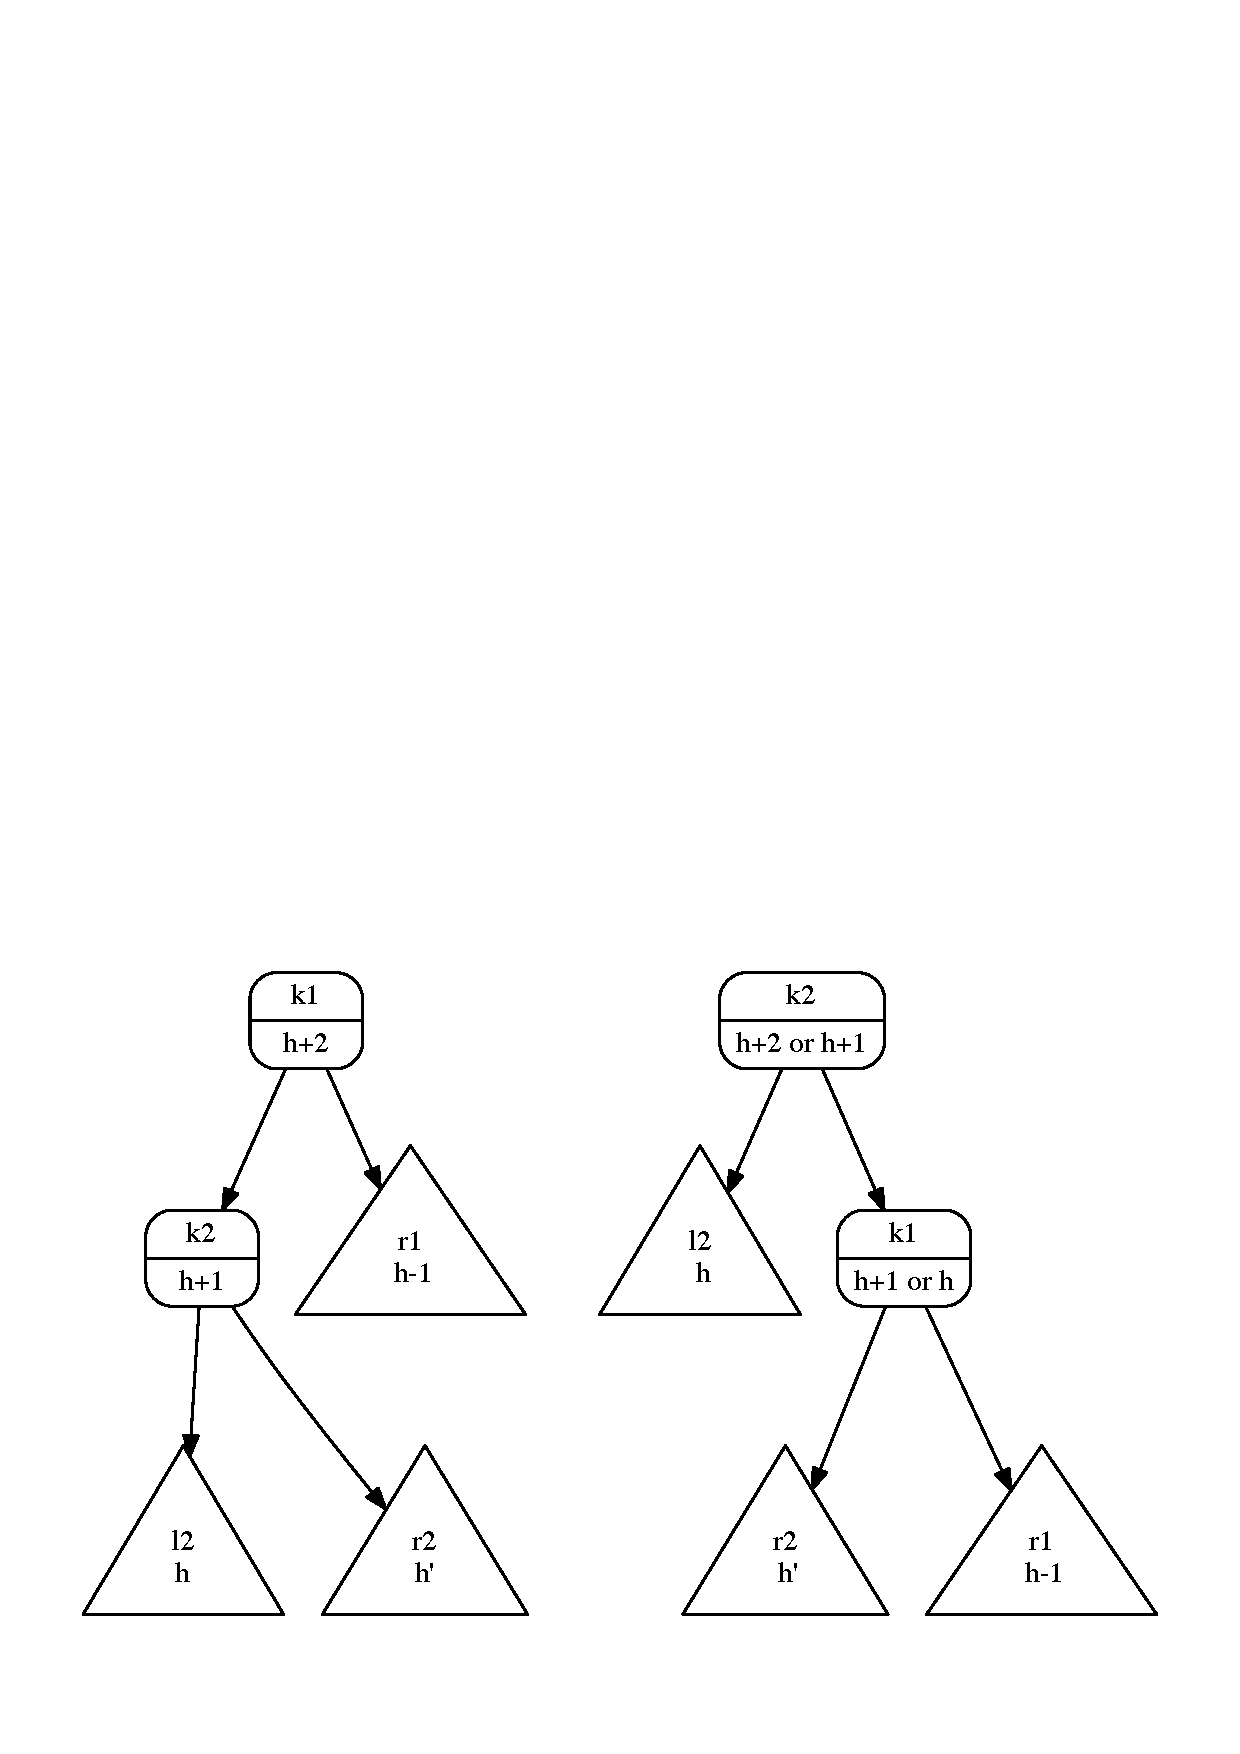
\epsfig{file=../casell,scale=0.9}} 
\vspace*{0.5cm}

$\begin{array}[t]{cl}
              & \textsl{height}(l_1) = \textsl{height}(r_1) + 2    \\[0.1cm] 
       \wedge & l_1 = \textsl{node}(k_2,v_2,l_2,r_2)               \\[0.1cm]
       \wedge & \textsl{height}(l_2) \geq \textsl{height}(r_2)     \\[0.3cm]
       \rightarrow & \quad \textsl{node}(k_1,v_1,l_1,r_1).\textsl{restore}() \\[0.1cm]
                   & = \textsl{node}\bigl(k_2,v_2,l_2,\textsl{node}(k_1,v_1,r_2,r_1)\bigr)
 \end{array}
$

\vspace*{\fill}
\tiny \addtocounter{mypage}{1}
\rule{17cm}{1mm}
 \hspace*{\fill} Seite \arabic{mypage}
\end{slide}

%%%%%%%%%%%%%%%%%%%%%%%%%%%%%%%%%%%%%%%%%%%%%%%%%%%%%%%%%%%%%%%%%%%%%%%%

\begin{slide}{}
\normalsize

\begin{center}
Implementierung von \textsl{restore}, 2. Fall
\end{center}
\vspace*{0.5cm}
\footnotesize
 \framebox{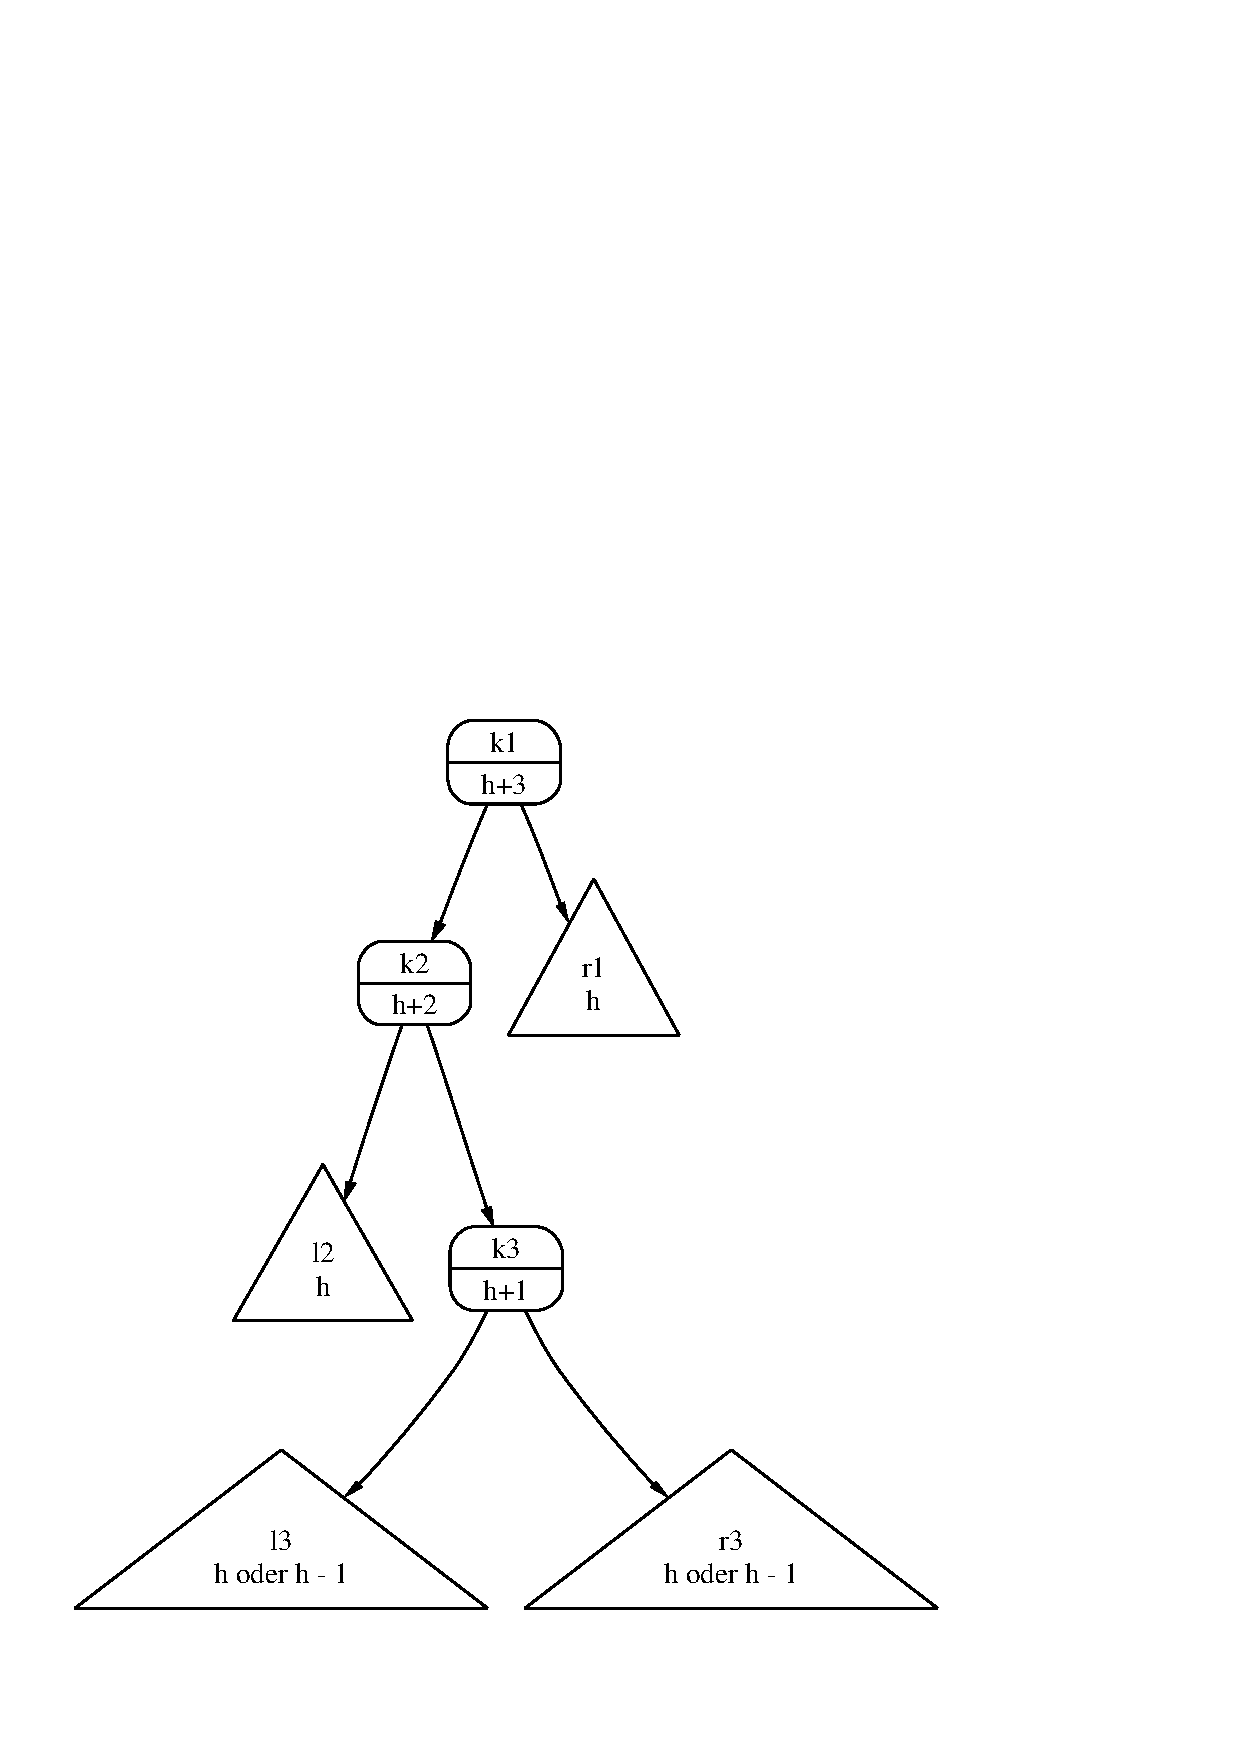
\epsfig{file=../caselr,scale=0.7}}  

 \framebox{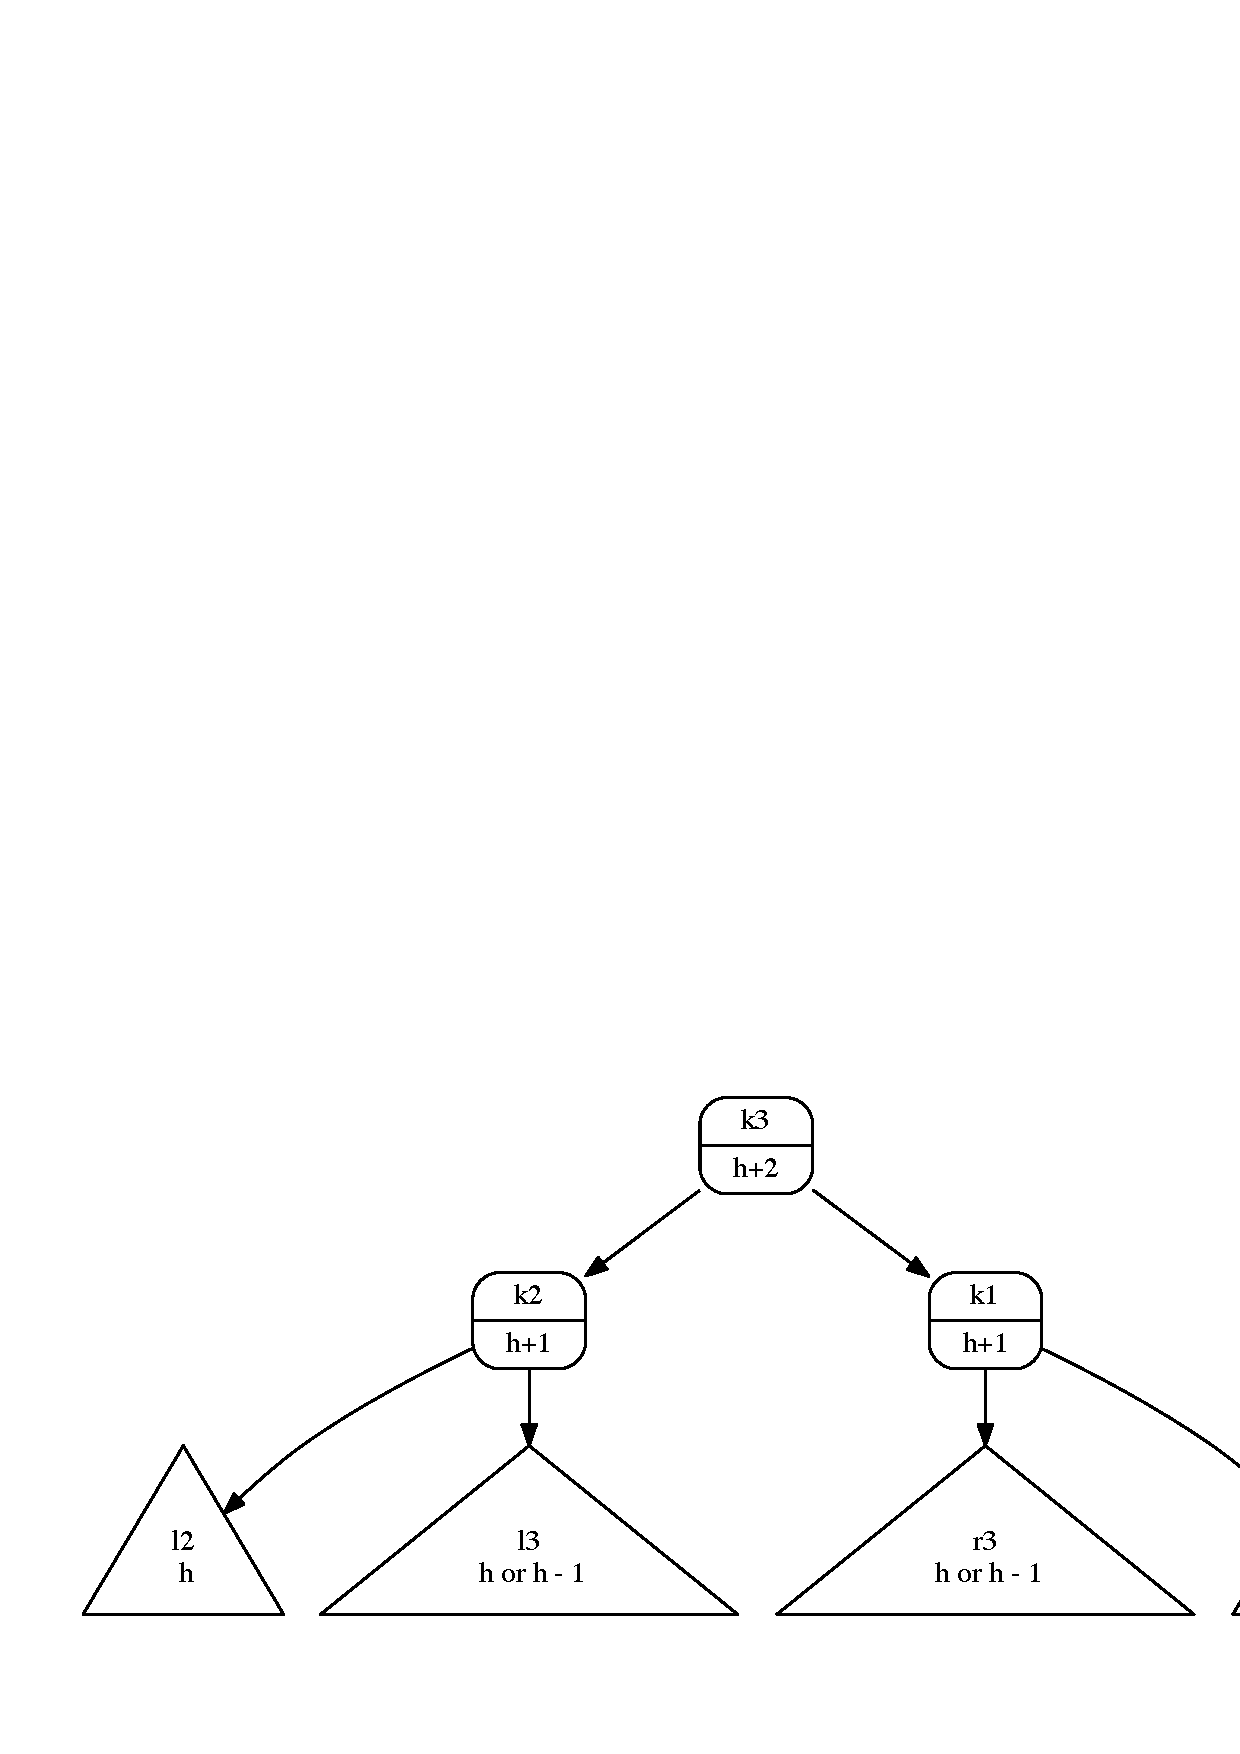
\epsfig{file=../caselr-nach,scale=0.7}} 

\vspace*{\fill}
\tiny \addtocounter{mypage}{1}
\rule{17cm}{1mm}
 \hspace*{\fill} Seite \arabic{mypage}
\end{slide}

%%%%%%%%%%%%%%%%%%%%%%%%%%%%%%%%%%%%%%%%%%%%%%%%%%%%%%%%%%%%%%%%%%%%%%%%

\begin{slide}{}
\normalsize

\begin{center}
AVL-B\"aume
\end{center}

\footnotesize
\begin{enumerate}
\item $\textsl{nil}\mathtt{.}\textsl{insert}(k,v) = \textsl{node}(k,v, \textsl{nil}, \textsl{nil})$.  
\item $\textsl{node}(k, v_2, l, r)\mathtt{.}\textsl{insert}(k,v_1) = \textsl{node}(k, v_1, l, r)$.
\item $k_1 < k_2 \;\rightarrow\; \textsl{node}(k_2, v_2, l, r)\mathtt{.}\textsl{insert}(k_1, v_1) =$ \\[0.1cm]
      \hspace*{3.1cm} 
      $\textsl{node}\bigl(k_2, v_2, l\mathtt{.}\textsl{insert}(k_1, v_1), r\bigr).\textsl{restore}()$.
\item $k_1 > k_2 \;\rightarrow \; \textsl{node}(k_2, v_2, l, r)\mathtt{.}\textsl{insert}(k_1, v_1) =$ \\[0.1cm]
      \hspace*{3.1cm}  
      $\textsl{node}\bigl(k_2, v_2, l, r\mathtt{.}\textsl{insert}(k_1, v_1)\bigr).\textsl{restore}()$.
\item $\textsl{node}(k, v, \textsl{nil}, r)\mathtt{.}\textsl{delMin}() = [r, k, v]$.
\item $l\not= \textsl{nil} \wedge l\mathtt{.}\textsl{delMin}() = [l',k_{min}, v_{min}] \;\rightarrow$ \\[0.1cm]
       \hspace*{3.1cm} 
       $\textsl{node}(k, v, l, r)\mathtt{.}\textsl{delMin}() \;=$ \\[0.1cm]
       \hspace*{3.1cm} 
       $[\textsl{node}(k, v, l', r).\textsl{restore}(), k_{min}, v_{min}]$.
\item $\textsl{nil}\mathtt{.}\textsl{delete}(k) = \textsl{nil}$.
\item $\textsl{node}(k,v,\textsl{nil},r)\mathtt{.}\textsl{delete}(k) = r$.
\item $\textsl{node}(k,v,l,\textsl{nil})\mathtt{.}\textsl{delete}(k) = l$.
\item $l \not= \textsl{nil} \,\wedge\, r \not= \textsl{nil} \,\wedge\, r\mathtt{.}\textsl{delMin}() = [r',k_{min}, v_{min}]  \;\rightarrow$ \\[0.1cm]
      $\textsl{node}(k,v,l,r)\mathtt{.}\textsl{delete}(k) = \textsl{node}(k_{min},v_{min},l,r').\textsl{restore}()$.
\item $k_1 < k_2 \;\rightarrow\; \textsl{node}(k_2,v_2,l,r)\mathtt{.}\textsl{delete}(k_1) =$ \\[0.1cm]
       \hspace*{3.1cm} 
      $\textsl{node}\bigl(k_2,v_2,l\mathtt{.}\textsl{delete}(k_1),r\bigr).\textsl{restore}()$.
\item $k_1 > k_2 \;\rightarrow\; \textsl{node}(k_2,v_2,l,r)\mathtt{.}\textsl{delete}(k_1) =$ \\[0.1cm]
       \hspace*{3.1cm} 
      $\textsl{node}\bigl(k_2,v_2,l,r\mathtt{.}\textsl{delete}(k_1)\bigr).\textsl{restore}()$.
\end{enumerate}


\vspace*{\fill}
\tiny \addtocounter{mypage}{1}
\rule{17cm}{1mm}
AVL-B\"aume \hspace*{\fill} Seite \arabic{mypage}
\end{slide}

%%%%%%%%%%%%%%%%%%%%%%%%%%%%%%%%%%%%%%%%%%%%%%%%%%%%%%%%%%%%%%%%%%%%%%%%

\begin{slide}{}
\normalsize

\begin{center}
Hash-Tabellen
\end{center}
\vspace*{0.5cm}

\footnotesize
\begin{verbatim}
    public class ArrayMap<Value> 
        implements MyMap<Integer, Value>
    {
        Value[] mArray;
        
        public ArrayMap(int n) {
            mArray = (Value[]) new Object[n+1];
        }
        public Value find(Integer key) {
            return mArray[key];
        }
        public void insert(Integer key, Value value) {
            mArray[key] = value;
        }
        public void delete(Integer key) {
            mArray[key] = null;
        }
    }
\end{verbatim}

\vspace*{\fill}
\tiny \addtocounter{mypage}{1}
\rule{17cm}{1mm}
\texttt{Hash-Tabellen} \hspace*{\fill} Seite \arabic{mypage}
\end{slide}

%%%%%%%%%%%%%%%%%%%%%%%%%%%%%%%%%%%%%%%%%%%%%%%%%%%%%%%%%%%%%%%%%%%%%%%

%%%%%%%%%%%%%%%%%%%%%%%%%%%%%%%%%%%%%%%%%%%%%%%%%%%%%%%%%%%%%%%%%%%%%%%%

\begin{slide}{}
\normalsize

\begin{center}
Abbildung von Namen auf Zahlen
\end{center}
\vspace*{0.5cm}

\footnotesize
\begin{enumerate}
\item Annahme: Namen haben L\"ange 8
      \begin{itemize}
      \item k\"urzere Namen mit Blanks auff\"ullen
      \item l\"angere Namen abschneiden
      \end{itemize}
\item Buchstaben als Ziffern $\{0, \cdots 26\}$ interpretieren:
  
      $\Sigma = \{ \texttt{' '}, \texttt{'a'}, \texttt{'b'}, \texttt{'c'}, \cdots, \texttt{'x'}, \texttt{'y'}, \texttt{'z'} \}$ 

      Funktion $\textsl{ord}: \Sigma \rightarrow \{0, \cdots s6\}$ definieren durch: 

      $\textsl{ord}(\texttt{' '}) = 0$, $\textsl{ord}(\texttt{'a'}) = 1$, 
      $\cdots$, $\textsl{ord}(\texttt{'z'}) = 26$.

\item Definiere $\textsl{code}: \Sigma^* \rightarrow \mathbb{N}$ \\[0.2cm]
      \hspace*{1.3cm} 
      $\textsl{code}(c_0c_1\cdots c_7) = \sum\limits_{i=0}^7 \textsl{ord}(c_i) \cdot 27^i$.
\end{enumerate}
Probleme: 
\begin{enumerate}
\item Gr\"o\3e des Feldes: \\[0.2cm]
      \hspace*{1.3cm} $(27^8-1) / 26 + 1 = 10\,862\,674\,481$ \\[0.2cm]
\item Funktion $\textsl{code}: \Sigma^* \rightarrow \mathbb{N}$ nicht bijektiv:
  
      nur die ersten 8 Buchstaben werden ber\"ucksichtigt.
\end{enumerate}

\vspace*{\fill}
\tiny \addtocounter{mypage}{1}
\rule{17cm}{1mm}
\texttt{Hash-Tabellen} \hspace*{\fill} Seite \arabic{mypage}
\end{slide}

%%%%%%%%%%%%%%%%%%%%%%%%%%%%%%%%%%%%%%%%%%%%%%%%%%%%%%%%%%%%%%%%%%%%%%%

%%%%%%%%%%%%%%%%%%%%%%%%%%%%%%%%%%%%%%%%%%%%%%%%%%%%%%%%%%%%%%%%%%%%%%%%

\begin{slide}{}
\normalsize

\begin{center}
Hash-Tabellen
\end{center}
\vspace*{0.5cm}

\footnotesize
  \framebox{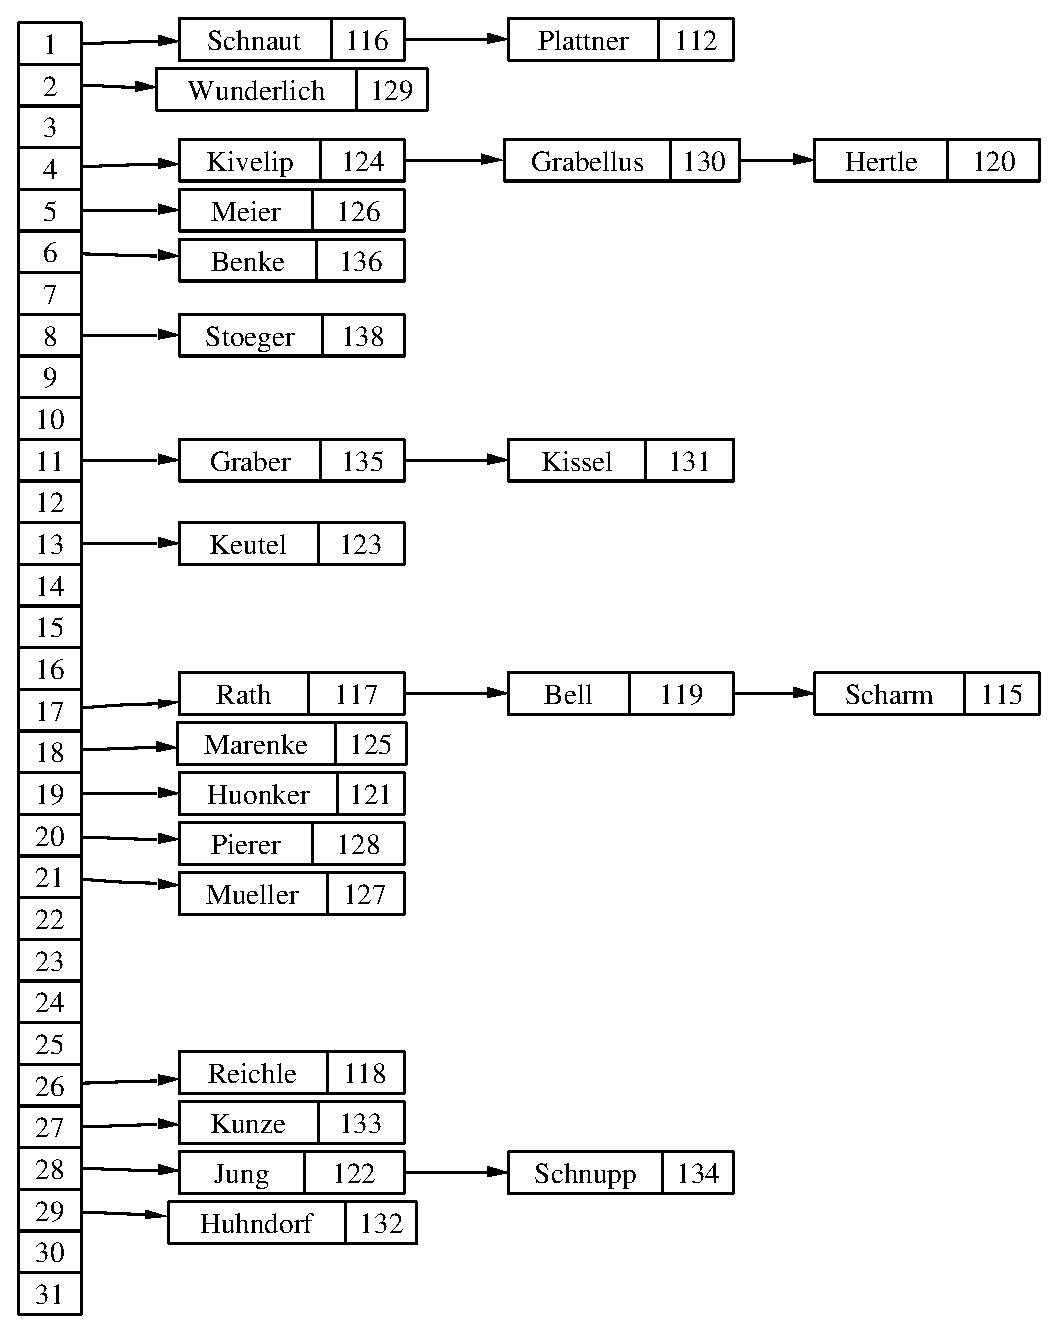
\epsfig{file=hash-table,scale=0.9}} 


\vspace*{\fill}
\tiny \addtocounter{mypage}{1}
\rule{17cm}{1mm}
\texttt{Hash-Tabellen} \hspace*{\fill} Seite \arabic{mypage}
\end{slide}

%%%%%%%%%%%%%%%%%%%%%%%%%%%%%%%%%%%%%%%%%%%%%%%%%%%%%%%%%%%%%%%%%%%%%%%

%%%%%%%%%%%%%%%%%%%%%%%%%%%%%%%%%%%%%%%%%%%%%%%%%%%%%%%%%%%%%%%%%%%%%%%%

\begin{slide}{}
\normalsize

\begin{center}
Mengen und Abbildungen in Java
\end{center}
\vspace*{0.5cm}

\footnotesize
Das Interface \texttt{Collection<E>}: \emph{Zusammenfassungen}
\begin{enumerate}
\item \texttt{boolean add(E $o$)}
  
      \begin{enumerate}
      \item $c.\mathtt{add}(e) \rightarrow c' = c \cup \{ e \}$

            $c'$: Wert der Zusammenfassungen nachher
      \item $c.\mathtt{add}(e) = (c' \not= c)$
      \end{enumerate}
\item \texttt{boolean addAll(Collection<E> $d$)} 

      \begin{enumerate}
      \item $c.\mathtt{addAll}(d) \rightarrow c' = c \cup d$,
      \item $c.\mathtt{addAll}(d) = (c' \not= c)$.
      \end{enumerate}
\item \texttt{void clear()}

      \hspace*{1.3cm} $c.\mathtt{clear}() \rightarrow c' = \{\}$.
\item \texttt{boolean contains(Element $e$)}

      \hspace*{1.3cm}
      $c.\mathtt{contains}(e) = (e \in c)$.
     
\item \texttt{boolean containsAll(Collection<E> $d$)}
        
      \hspace*{1.3cm}
      $c.\mathtt{containsAll}(d) = (d \subseteq c)$.
      
\item \texttt{boolean isEmpty()}

      \hspace*{1.3cm}
      $c.\mathtt{isEmpty}() = \bigl(c = \{\}\bigr)$.
\end{enumerate}

\vspace*{\fill}
\tiny \addtocounter{mypage}{1}
\rule{17cm}{1mm}
\texttt{Collection<E>} \hspace*{\fill} Seite \arabic{mypage}
\end{slide}

%%%%%%%%%%%%%%%%%%%%%%%%%%%%%%%%%%%%%%%%%%%%%%%%%%%%%%%%%%%%%%%%%%%%%%%

%%%%%%%%%%%%%%%%%%%%%%%%%%%%%%%%%%%%%%%%%%%%%%%%%%%%%%%%%%%%%%%%%%%%%%

\begin{slide}{}
\normalsize

\begin{center}
\texttt{Collection<E>}, Fortsetzung
\end{center}
\vspace*{0.5cm}

\footnotesize
\begin{enumerate}
\setcounter{enumi}{7}
\item \texttt{boolean remove(Object $e$)}

      \begin{enumerate}
      \item $c.\mathtt{remove}(e) \rightarrow c' = c \,\backslash\, \{ e \}$,
      \item $c.\mathtt{remove}(e) = (e \in c)$.
      \end{enumerate}
\item \texttt{boolean removeAll(Collection<?> $d$)}

      \begin{enumerate}
      \item $c.\mathtt{removeAll}(d) \rightarrow c' = c \,\backslash\, d$,
      \item $c.\mathtt{removeAll}(d) = \bigl(d \cap c \not= \{\}\bigr)$.
      \end{enumerate}
\item \texttt{boolean retainAll(Collection<?> $d$)}

      \begin{enumerate}
      \item $c.\mathtt{retainAll}(d) \rightarrow c' = c \cap d$,
      \item $c.\mathtt{retainAll}(d) = (d \subseteq c)$.
      \end{enumerate}
\item \texttt{int size()}

      $c.\mathtt{size}() = \# c$ \quad Anzahl der Elemente
\item \texttt{Object[] toArray()}
  
      Umwandlung: \texttt{Collection<T>} $\mapsto$ Feld 
\item \texttt{T[] toArray(T[] $a$)}

      Umwandlung: \texttt{Collection<T>} $\mapsto$ Feld vom Typ \texttt{T[]}

\end{enumerate}

\vspace*{\fill}
\tiny \addtocounter{mypage}{1}
\rule{17cm}{1mm}
\texttt{Collection<T>} \hspace*{\fill} Seite \arabic{mypage}
\end{slide}

%%%%%%%%%%%%%%%%%%%%%%%%%%%%%%%%%%%%%%%%%%%%%%%%%%%%%%%%%%%%%%%%%%%%%%%
%%%%%%%%%%%%%%%%%%%%%%%%%%%%%%%%%%%%%%%%%%%%%%%%%%%%%%%%%%%%%%%%%%%%%%

\begin{slide}{}
\normalsize

\begin{center}
Generische Felder
\end{center}
\vspace*{0.5cm}

\footnotesize

\begin{enumerate}
\item Keine generische Erzeugung von Feldern in Java:
      \\[0.2cm]
      \hspace*{1.3cm}
      \texttt{T[] a = new T[10];  // compile time error} 

\item Kein Casten von Feldern:
\begin{Verbatim}[ frame         = lines, 
                  framesep      = 0.3cm, 
                  labelposition = bottomline,
                  numbersep     = -0.2cm,
                  xleftmargin   = 0.0cm,
                  xrightmargin  = 0.0cm,
                ]
public class TestCast 
{ 
    public static void main(String[] args) {
        List<Integer> l = new LinkedList<Integer>();
        for (Integer i = 0; i < 10; ++i) {
            l.add(i);
        }
        Object [] a = l.toArray();
        Integer[] b = (Integer[]) a;
    }
}
\end{Verbatim}
Exception: \texttt{ClassCastException}
\end{enumerate}

\vspace*{\fill}
\tiny \addtocounter{mypage}{1}
\rule{17cm}{1mm}
Generische Felder \hspace*{\fill} Seite \arabic{mypage}
\end{slide}

%%%%%%%%%%%%%%%%%%%%%%%%%%%%%%%%%%%%%%%%%%%%%%%%%%%%%%%%%%%%%%%%%%%%%%%

%%%%%%%%%%%%%%%%%%%%%%%%%%%%%%%%%%%%%%%%%%%%%%%%%%%%%%%%%%%%%%%%%%%%%%

\begin{slide}{}
\normalsize

\begin{center}
Generische Felder
\end{center}
\vspace*{0.5cm}

\footnotesize
Erzeugung generischer Felder:
\begin{Verbatim}[ frame         = lines, 
                  framesep      = 0.3cm, 
                  labelposition = bottomline,
                  numbersep     = -0.2cm,
                  xleftmargin   = 0.0cm,
                  xrightmargin  = 0.0cm,
                ]
public class TestCast2 
{
    public static void main(String[] args) {
        List<Integer> l = new LinkedList<Integer>();
        for (Integer i = 0; i < 10; ++i) {
            l.add(i);
        }
        Integer[] a = new Integer[0];
        Integer[] b = l.toArray(a);
    }
}
\end{Verbatim}


\vspace*{\fill}
\tiny \addtocounter{mypage}{1}
\rule{17cm}{1mm}
Generische Felder \hspace*{\fill} Seite \arabic{mypage}
\end{slide}

%%%%%%%%%%%%%%%%%%%%%%%%%%%%%%%%%%%%%%%%%%%%%%%%%%%%%%%%%%%%%%%%%%%%%%%

%%%%%%%%%%%%%%%%%%%%%%%%%%%%%%%%%%%%%%%%%%%%%%%%%%%%%%%%%%%%%%%%%%%%%%

\begin{slide}{}
\normalsize

\begin{center}
\texttt{Collection<E>}, Fortsetzung
\end{center}
\vspace*{0.5cm}

\footnotesize
\begin{enumerate}
\setcounter{enumi}{13}
\item \texttt{Iterator<E> iterator()}

      $c.\mathtt{iterator}()$ liefert Iterator f\"ur Zusammenfassungen $c$

      erm\"oglicht erweiterte \texttt{for}-Schleife
      \\[0.2cm]
      \hspace*{1.3cm} \texttt{for (E e: c) \{} \\
      \hspace*{2.3cm} \texttt{System.out.println(e);} \\
      \hspace*{1.3cm} \texttt{\}} 
\end{enumerate}
\vspace*{0.5cm}

\begin{center}
Schnittstelle \texttt{Iterator<E>}
\end{center}
\vspace*{0.5cm}

\begin{enumerate}
\item \texttt{boolean hasNext()}

      noch nicht alle Elemente aufgez\"ahlt
\item \texttt{E next()}

      liefert n\"achstes Element
\item \texttt{void remove()}

      entfernt zuletzt geliefertes Element 
\end{enumerate}

\vspace*{\fill}
\tiny \addtocounter{mypage}{1}
\rule{17cm}{1mm}
\texttt{Collection<E>} \hspace*{\fill} Seite \arabic{mypage}
\end{slide}

%%%%%%%%%%%%%%%%%%%%%%%%%%%%%%%%%%%%%%%%%%%%%%%%%%%%%%%%%%%%%%%%%%%%%%%

%%%%%%%%%%%%%%%%%%%%%%%%%%%%%%%%%%%%%%%%%%%%%%%%%%%%%%%%%%%%%%%%%%%%%%

\begin{slide}{}
\normalsize

\begin{center}
 \texttt{Set<E> implements Collection<E>}
\end{center}
\vspace*{0.5cm}

\footnotesize
Implementierung: \texttt{TreeSet<E>}

Bedingung: Elemente vergleichbar
\begin{enumerate}
\item \texttt{E first()}

      $s.\mathtt{first}()$: \quad kleinstes Element von $s$
\item \texttt{E last()}

      $s.\mathtt{last}()$: \quad gr\"o\3tes Element von $s$.
\end{enumerate}
Konstruktoren
\begin{enumerate}
\item \texttt{TreeSet()}: \quad leere Menge
\item \texttt{TreeSet(Collection<E> $c$)}
  
      alle Elemente aus $c$ 
\end{enumerate}
\vspace*{0.5cm}

\begin{center}
Implementierung: Rot-Schwarz-B\"aume  
\end{center}


\vspace*{\fill}
\tiny \addtocounter{mypage}{1}
\rule{17cm}{1mm}
\texttt{TreeSet<E>} \hspace*{\fill} Seite \arabic{mypage}
\end{slide}

%%%%%%%%%%%%%%%%%%%%%%%%%%%%%%%%%%%%%%%%%%%%%%%%%%%%%%%%%%%%%%%%%%%%%%%

%%%%%%%%%%%%%%%%%%%%%%%%%%%%%%%%%%%%%%%%%%%%%%%%%%%%%%%%%%%%%%%%%%%%%%

\begin{slide}{}
\normalsize

\begin{center}
Rot-Schwarz-B\"aume
\end{center}
\vspace*{0.5cm}

\footnotesize
\begin{enumerate}
\item N\"aherungsweise balancierte bin\"are B\"aume.
\item Knoten markiert: rot oder schwarz
\item Wurzel: schwarz.
\item Kinder eines roten Knotens: schwarz. 
\item Kinder eines schwarzen Knotens: rot oder schwarz.  
\item H\"ohe:  rote Knoten werden nicht gez\"ahlt.
\item Linker und rechter Teil-Baum: selbe H\"ohe.
\end{enumerate}

Komplexit\"at
\begin{enumerate}
\item $\textsl{find}()$:   \quad $\Oh\bigl(\log(n)\bigr)$
\item $\textsl{insert}()$: \quad $\Oh\bigl(\log(n)\bigr)$
\item $\textsl{delete}()$: \quad $\Oh\bigl(\log(n)\bigr)$
\end{enumerate}


\vspace*{\fill}
\tiny \addtocounter{mypage}{1}
\rule{17cm}{1mm}
 \hspace*{\fill} Seite \arabic{mypage}
\end{slide}

%%%%%%%%%%%%%%%%%%%%%%%%%%%%%%%%%%%%%%%%%%%%%%%%%%%%%%%%%%%%%%%%%%%%%%%

%%%%%%%%%%%%%%%%%%%%%%%%%%%%%%%%%%%%%%%%%%%%%%%%%%%%%%%%%%%%%%%%%%%%%%

\begin{slide}{}
\normalsize

\begin{center}
\texttt{HashSet<E>}
\end{center}
\vspace*{0.5cm}

\footnotesize
\begin{enumerate}
\item \texttt{HashSet()}: \quad leere Hash-Tabelle.  

      Load-Faktor: $0.75$ 

      Initiale Gr\"o\3e des Feldes: 16
\item \texttt{HashSet(Collection<E> $c$)}

      Load-Faktor: $0.75$.
\item \texttt{HashSet(int $n$)}
  
      Initiale Gr\"o\3e: $n$.  

      Load-Faktor: $0.75$.
\item \texttt{HashSet(int $n$, float $\alpha$)}

      Initiale Gr\"o\3e: $n$.  

      Load-Faktor: $\alpha$.
\end{enumerate}



\vspace*{\fill}
\tiny \addtocounter{mypage}{1}
\rule{17cm}{1mm}
\texttt{HashSet<E>} \hspace*{\fill} Seite \arabic{mypage}
\end{slide}

%%%%%%%%%%%%%%%%%%%%%%%%%%%%%%%%%%%%%%%%%%%%%%%%%%%%%%%%%%%%%%%%%%%%%%%

%%%%%%%%%%%%%%%%%%%%%%%%%%%%%%%%%%%%%%%%%%%%%%%%%%%%%%%%%%%%%%%%%%%%%%

\begin{slide}{}
\normalsize

\begin{center}
\texttt{List<E> implements Set<E>}
\end{center}

\footnotesize
zus\"atzlich: Index
\begin{enumerate}
\item \texttt{E get(int $i$)}

      $l.\mathtt{get}(i)$: \quad $i$-tes Element von $l$
\item \texttt{void set(int $i$, E $e$)}      

      $l.\mathtt{set}(i, e)$: \quad ersetze $i$-te Element.
\item \texttt{add}, \texttt{addAll}: 

      Einf\"ugen am Ende der Liste
\item \texttt{void add(int $i$, E $e$)}

      Einf\"ugen an Position $i$ 
\item \texttt{void addAll(int $i$, Collection<E> $c$)}

      Einf\"ugen an Position $i$ 
\end{enumerate}

Implementierungen
\begin{enumerate}
\item \texttt{LinkedList}: \quad verkettete Listen

      Komplexit\"at $l.\mathtt{get}(i)$, $l.\mathtt{set}(i,e)$: \quad linear

      Komplexit\"at $l.\mathtt{add}(e)$: \hspace*{3.5cm} konstant
\item \texttt{ArrayList}: \quad Feld

      Komplexit\"at $l.\mathtt{get}(i)$, $l.\mathtt{set}(i,e)$: \quad konstant

      Komplexit\"at $l.\mathtt{add}(0,e)$: \hspace*{2.9cm} linear
\end{enumerate}

\vspace*{\fill}
\tiny \addtocounter{mypage}{1}
\rule{17cm}{1mm}
\texttt{List<E>} \hspace*{\fill} Seite \arabic{mypage}
\end{slide}

%%%%%%%%%%%%%%%%%%%%%%%%%%%%%%%%%%%%%%%%%%%%%%%%%%%%%%%%%%%%%%%%%%%%%%%

%%%%%%%%%%%%%%%%%%%%%%%%%%%%%%%%%%%%%%%%%%%%%%%%%%%%%%%%%%%%%%%%%%%%%%

\begin{slide}{}
\normalsize

\begin{center}
\texttt{Queue<E> implements Collection<E>}
\end{center}
\vspace*{0.5cm}

\footnotesize
\begin{enumerate}
\item \texttt{E element()}
  
      $q.\mathtt{element}()$: erstes Element 

      $q$ wird nicht ver\"andert

      $q$ leer, dann \texttt{NoSuchElementException} 
\item \texttt{boolean offer(E $e$)}

      $q.\mathtt{offer}(e)$: \quad einf\"ugen von e $e$ am Ende

      $q$ voll:  \texttt{false}, sonst \texttt{true}.
\item \texttt{E peek()}

      $q.\mathtt{element}()$: erstes Element 

      $q$ wird nicht ver\"andert

      $q$ leer: Ergebnis \texttt{null} 
\item \texttt{E poll()}

      $q.\mathtt{poll}()$:  erstes Element 

      Element wird entfernt

      $q$ leer: Ergebnis \texttt{null} 
      Warteschlange leer ist, wird \texttt{null} zur\"uck gegeben.
\item \texttt{E remove()}

      $q.\mathtt{remove}()$: erstes Element 

      Element wird entfernt

      $q$ leer: \texttt{NoSuchElementException}
\end{enumerate}


\vspace*{\fill}
\tiny \addtocounter{mypage}{1}
\rule{17cm}{1mm}
\texttt{Queue<E>} \hspace*{\fill} Seite \arabic{mypage}
\end{slide}

%%%%%%%%%%%%%%%%%%%%%%%%%%%%%%%%%%%%%%%%%%%%%%%%%%%%%%%%%%%%%%%%%%%%%%%

%%%%%%%%%%%%%%%%%%%%%%%%%%%%%%%%%%%%%%%%%%%%%%%%%%%%%%%%%%%%%%%%%%%%%%

\begin{slide}{}
\normalsize

\begin{center}
Abbildungen: \texttt{Map<K,V>}
\end{center}
\vspace*{0.5cm}

\footnotesize
\begin{enumerate}
\item \texttt{V get(K $k$)}
  
      entspricht $\texttt{find}()$
\item \texttt{boolean containsKey(K $k$)}

      $m.\mathtt{containsKey}(k) \approx (\exists k: m.\mathtt{get}(k) \not= \mathtt{null})$
\item \texttt{V put(K $k$, V $v$)}

      entspricht $\texttt{insert}()$ 
\item \texttt{V remove(K $k$)}
  
      entspricht  $\texttt{delete}()$ 
\item \texttt{void clear()}

      l\"oscht alle Zuordnungen
\item \texttt{boolean containsValue(V $v$)}

      $m.\mathtt{containsValue}(v) \leftrightarrow \Bigl(\exists k: m.\mathtt{get}(k) = v\Bigr)$

      Komplexit\"at: linear 
\item \texttt{boolean isEmpty()}
  
\end{enumerate}


\vspace*{\fill}
\tiny \addtocounter{mypage}{1}
\rule{17cm}{1mm}
\texttt{Map<K,V>} \hspace*{\fill} Seite \arabic{mypage}
\end{slide}

%%%%%%%%%%%%%%%%%%%%%%%%%%%%%%%%%%%%%%%%%%%%%%%%%%%%%%%%%%%%%%%%%%%%%%

\begin{slide}{}
\normalsize

\begin{center}
\texttt{Map<K,V>}, Fortsetzung
\end{center}
\vspace*{0.5cm}

\footnotesize
\begin{enumerate}
\setcounter{enumi}{7}
 \item \texttt{Set<K> keySet()}

      $m.\mathtt{keySet}() = \{ k \mid m.\mathtt{get}(k) \not= \mathtt{null} \}$
      \vspace*{0.3cm}

      \emph{Ansicht} der Schl\"ussel (engl. \emph{view})
      \begin{enumerate}
      \item L\"oschen in $m.\mathtt{keySet}()$

            Zuordnung verschwindet aus $m$
      \item kein Einf\"ugen: 

            $m.\mathtt{keySet}().\mathtt{add}(x) \mapsto \texttt{UnsupportedOperationException}$
      \end{enumerate}

\item \texttt{Collection<V> values()}

      Ansicht der Werte

      $m.\mathtt{values}() = \{ v \mid \exists k: m.\mathtt{get}(k) = v \}$

      L\"oschen erlaubt, Einf\"ugen nicht
\item \texttt{void putAll(Map<K,V> $t$)}

      $m.\mathtt{putAll}(t) \approx m \cup t$ 

      Zuordnungen aus $t$ \"uberschreiben Zuordnungen aus $m$
\item \texttt{int size()}

      $m.\mathtt{size}() = \#\{ k \mid m.\mathtt{get}(k) \not= \mathtt{null} \}$
\end{enumerate}

\vspace*{\fill}
\tiny \addtocounter{mypage}{1}
\rule{17cm}{1mm}
\texttt{Map<K,V>} \hspace*{\fill} Seite \arabic{mypage}
\end{slide}

%%%%%%%%%%%%%%%%%%%%%%%%%%%%%%%%%%%%%%%%%%%%%%%%%%%%%%%%%%%%%%%%%%%%%%%

%%%%%%%%%%%%%%%%%%%%%%%%%%%%%%%%%%%%%%%%%%%%%%%%%%%%%%%%%%%%%%%%%%%%%%

\begin{slide}{}
\normalsize

\begin{center}
\texttt{TreeMap<K,V> implements Map<K,V>}
\end{center}
\vspace*{0.5cm}

\footnotesize
Bedingung:  Schl\"ussel geordnet
\begin{enumerate}
\item nat\"urlicher Vergleich: \quad \texttt{K implements Comparable<K>}

      \hspace*{1.3cm} $k_1.\mathtt{compareTo}(k_2)$

      \begin{enumerate}
      \item $k_1 < k_2 \leftrightarrow k_1.\mathtt{compareTo}(k_2) < 0$
      \item $k_1 = k_2 \leftrightarrow k_1.\mathtt{compareTo}(k_2) = 0$
      \item $k_1 > k_2 \leftrightarrow k_1.\mathtt{compareTo}(k_2) > 0$
      \end{enumerate}
\item \emph{Komparator-Objekt} 

      $c.\mathtt{compare}(o_1, o_2)$
\end{enumerate}

 Konstruktoren
\begin{enumerate}
\item \texttt{TreeMap()}
\item \texttt{TreeMap(Comparator<K> $c$)}
\item \texttt{TreeMap(Map<K,V> $m$)}
\end{enumerate}


\vspace*{\fill}
\tiny \addtocounter{mypage}{1}
\rule{17cm}{1mm}
\texttt{TreeMap} \hspace*{\fill} Seite \arabic{mypage}
\end{slide}

%%%%%%%%%%%%%%%%%%%%%%%%%%%%%%%%%%%%%%%%%%%%%%%%%%%%%%%%%%%%%%%%%%%%%%%
%%%%%%%%%%%%%%%%%%%%%%%%%%%%%%%%%%%%%%%%%%%%%%%%%%%%%%%%%%%%%%%%%%%%%%

\begin{slide}{}
\normalsize

\begin{center}
\texttt{HashMap<K,V> implements Map<K,V>}
\end{center}
\vspace*{0.5cm}

\footnotesize
\begin{enumerate}
\item \texttt{HashMap()}
  
      leere Hash-Tabelle.  

      Load-Faktor: $0.75$ 

      initiale Gr\"o\3e: 16
\item \texttt{HashMap(int $n$)}
  
      leere Hash-Tabelle.  

      Load-Faktor: $0.75$ 

      initiale Gr\"o\3e: $n$
\item \texttt{HashMap(int $n$, float $\alpha$)}

      leere Hash-Tabelle.  

      Load-Faktor: $\alpha$ 

      initiale Gr\"o\3e: $n$
\item \texttt{HashMap(Map<K,V> $m$)}

      Load-Faktor: $0.75$ 
\end{enumerate}


\vspace*{\fill}
\tiny \addtocounter{mypage}{1}
\rule{17cm}{1mm}
Priorit\"ats-Warteschlangen \hspace*{\fill} Seite \arabic{mypage}
\end{slide}

%%%%%%%%%%%%%%%%%%%%%%%%%%%%%%%%%%%%%%%%%%%%%%%%%%%%%%%%%%%%%%%%%%%%%%

\begin{slide}{}
\normalsize

\begin{center}
Priorit\"ats-Warteschlangen
\end{center}
\vspace*{0.5cm}

\footnotesize
\begin{enumerate}

\item Namen: \quad \textsl{PrioQueue}.
\item Typ-Parameter: \quad $\{ \textsl{Key}, \textsl{Value} \}$.

      $\langle \textsl{Key}, \leq \rangle$: \quad totale Quasi-Ordnung
\item Funktions-Zeichen:\\[0.1cm]
     \hspace*{1.3cm} 
     $\{ \textsl{PrioQueue}, \textsl{insert}, \textsl{remove}, \textsl{top}, \textsl{change} \}$.
\item Typ-Spezifikationen:
      \begin{enumerate}
      \item $\textsl{PrioQueue}: \textsl{PrioQueue}$
      \item $\textsl{top}: \textsl{PrioQueue} \rightarrow 
             (\textsl{Key} \times \textsl{Value}) \cup \{\Omega\}$
      \item $\textsl{insert}: \textsl{PrioQueue} \times \textsl{Key} \times \textsl{Value}
            \rightarrow \textsl{PrioQueue}$
      \item $\textsl{remove}: \textsl{PrioQueue} \rightarrow \textsl{PrioQueue}$
      \item $\textsl{change}: \textsl{PrioQueue} \times \textsl{Key} \times \textsl{Value}
             \rightarrow \textsl{PrioQueue}$
      \end{enumerate}
\end{enumerate}


\vspace*{\fill}
\tiny \addtocounter{mypage}{1}
\rule{17cm}{1mm}
 \hspace*{\fill} Seite \arabic{mypage}
\end{slide}

%%%%%%%%%%%%%%%%%%%%%%%%%%%%%%%%%%%%%%%%%%%%%%%%%%%%%%%%%%%%%%%%%%%%%%

\begin{slide}{}
\normalsize

\begin{center}
Priorit\"ats-Warteschlangen --- Axiome \\[0.4cm]
Referenz-Implementierung
\end{center}
\vspace*{0.5cm}

\footnotesize
\begin{enumerate}
\setcounter{enumi}{4}

\item $\textsl{new PrioQueue}() = \{\}$
\item $Q.\textsl{insert}(k, v) = Q \cup \biggl\{ \pair(k,v) \biggr\}$
\item $Q = \{\} \;\rightarrow\; Q.\textsl{top}() = \Omega$
\item $\pair(k_1,v_1) \in Q \;\wedge\; Q.\textsl{top}() = \pair(k_2,v_2) \;\rightarrow\; $ \\[0.3cm]
      \hspace*{2cm} $k_2 \leq k_1 \;\wedge\; \pair(k_2,v_2) \in Q$
\item $Q = \{\} \rightarrow Q.\textsl{remove}() = Q$
\item $Q \not= \{\} \rightarrow Q.\textsl{remove}() = Q \backslash \biggl\{ Q.\textsl{top}() \biggr\}$
\item $Q.\textsl{change}(k_1,v_1) = 
       \biggl\{ \pair(k_2,v_2) \in Q \mid v_2 \not= v_1 \biggr\} \cup \biggl\{ \pair(k_1,v_1) \biggr\}$
\end{enumerate}

Einfache Implementierungen: \quad geordnete Liste

Komplexit\"at von $Q.\textsl{insert}(k,v)$: \quad $\Oh(\#Q)$

\vspace*{\fill}
\tiny \addtocounter{mypage}{1}
\rule{17cm}{1mm}
Priorit\"ats-Warteschlangen: Verhalten \hspace*{\fill} Seite \arabic{mypage}
\end{slide}

%%%%%%%%%%%%%%%%%%%%%%%%%%%%%%%%%%%%%%%%%%%%%%%%%%%%%%%%%%%%%%%%%%%%%%

\begin{slide}{}
\normalsize

\begin{center}
Daten-Struktur \textsl{Heap}
\end{center}
\vspace*{0.5cm}

\footnotesize
\hspace*{1.2cm}  $\leq: \textsl{Key} \times \mathcal{B} \rightarrow \mathbb{B}$
\begin{enumerate}
\item $k_1 \leq \textsl{nil}$
\item $k_1 \leq \textsl{node}(k_2,v,l,r) 
       \;\stackrel{\mbox{\scriptsize def}}{\longleftrightarrow}\; 
       k_1 \leq k_2 \;\wedge\; k_1 \leq l \;\wedge\; k_2 \leq r$         
\end{enumerate}

\hspace*{1.2cm}  $\textsl{count}: \mathcal{B} \rightarrow \mathbb{N}$
\begin{enumerate}
\item $\textsl{nil}.\textsl{count}() = 0$.
\item $\textsl{node}(k,v,l,r).\textsl{count}() = 1 + l.\textsl{count}() + r.\textsl{count}()$.
\end{enumerate}

Induktive Definition von $\textsl{Heap} \subseteq \mathcal{B}$
\begin{enumerate}
\item $\textsl{nil} \in \textsl{Heap}$.
\item $\textsl{node}(k,v,l,r) \in \textsl{Heap}$ g.d.w. folgendes gilt:
      \begin{enumerate}
      \item \emph{Heap-Bedingung}

            $k \leq l \;\wedge\; k \leq r$ 
      \item \emph{Balancierungs-Bedingung}

            $\mid l.\textsl{count}() - r.\textsl{count}() \mid \;\leq\, 1$
      \item $l \in \textsl{Heap} \;\wedge\; r \in \textsl{Heap}$.
      \end{enumerate}
\end{enumerate}



\vspace*{\fill}
\tiny \addtocounter{mypage}{1}
\rule{17cm}{1mm}
 \hspace*{\fill} Seite \arabic{mypage}
\end{slide}

%%%%%%%%%%%%%%%%%%%%%%%%%%%%%%%%%%%%%%%%%%%%%%%%%%%%%%%%%%%%%%%%%%%%%%%

\begin{slide}{}
\normalsize

\begin{center}
Heap --- Beispiel
\end{center}
\vspace*{0.5cm}

\footnotesize
  \framebox{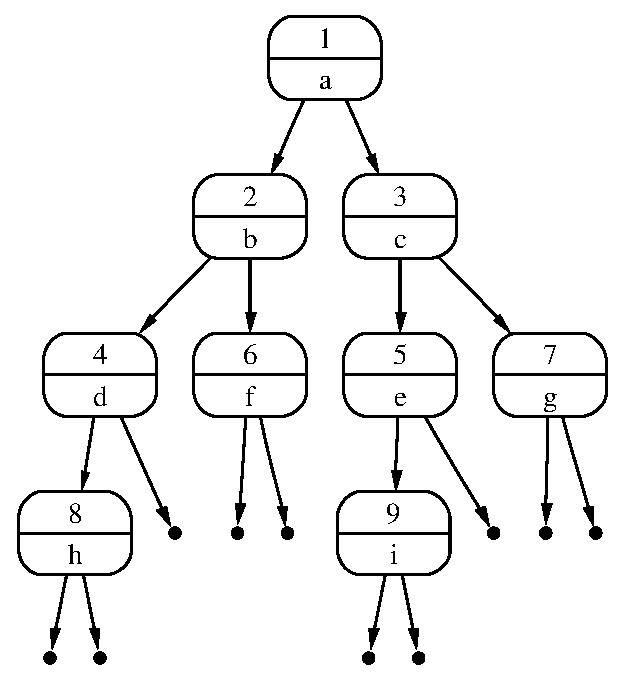
\epsfig{file=../heap-with-holes,scale=1.6}} 

\vspace*{\fill}
\tiny \addtocounter{mypage}{1}
\rule{17cm}{1mm}
Heap --- Beispiel \hspace*{\fill} Seite \arabic{mypage}
\end{slide}

%%%%%%%%%%%%%%%%%%%%%%%%%%%%%%%%%%%%%%%%%%%%%%%%%%%%%%%%%%%%%%%%%%%%%%%

\begin{slide}{}
\normalsize

\begin{center}
Heap --- Implementierung
\end{center}
\vspace*{0.5cm}


\footnotesize
$\textsl{top}:\textsl{Heap} \rightarrow (\textsl{Key} \times \textsl{Value}) \cup \Omega$
\begin{enumerate}
\item $\textsl{nil}.\textsl{top}() = \Omega$
\item $\textsl{node}(k,v,l,r).\textsl{top}() = \pair(k,v)$
\end{enumerate}

$\textsl{insert}: \textsl{Heap} \times \textsl{Key} \times \textsl{Value} \rightarrow \textsl{Heap}$
\begin{enumerate}
\item $\textsl{nil}.\textsl{insert}(k,v) = \textsl{node}(k,v,\textsl{nil}, \textsl{nil})$.
\item $k_{\mathrm{top}} \leq k \;\wedge\; l.\textsl{count}() \leq r.\textsl{count}() \;\rightarrow $ \\[0.3cm]
      $\textsl{node}(k_{\mathrm{top}},v_\mathrm{top},l,r).\textsl{insert}(k,v) =$ \\[0.3cm]
      $\textsl{node}\bigl(k_\mathrm{top},v_\mathrm{top},l.\textsl{insert}(k,v), r\bigr)$.

\item $k_{\mathrm{top}} \leq k \;\wedge\; l.\textsl{count}() > r.\textsl{count}() \;\rightarrow $ \\[0.3cm]
      $\textsl{node}(k_{\mathrm{top}},v_\mathrm{top},l,r).\textsl{insert}(k,v) =$ \\[0.3cm]
      $\textsl{node}\bigl(k_\mathrm{top},v_\mathrm{top},l,r.\textsl{insert}(k,v)\bigr)$.

\item $k_{\mathrm{top}} > k \;\wedge\; l.\textsl{count}() \leq r.\textsl{count}() \;\rightarrow $ \\[0.3cm]
      $\textsl{node}(k_{\mathrm{top}},v_\mathrm{top},l,r).\textsl{insert}(k,v) =$ \\[0.3cm]
      $\textsl{node}\bigl(k,v,l.\textsl{insert}(k_\mathrm{top},v_\mathrm{top}), r\bigr)$.
\item $k_{\mathrm{top}} > k \;\wedge\; l.\textsl{count}() > r.\textsl{count}() \;\rightarrow $ \\[0.3cm] 
      $\textsl{node}(k_{\mathrm{top}},v_\mathrm{top},l,r).\textsl{insert}(k,v) =$ \\[0.3cm]
      $\textsl{node}\bigl(k,v,l,r.\textsl{insert}(k_\mathrm{top},v_\mathrm{top})\bigr)$.
\end{enumerate}


\vspace*{\fill}
\tiny \addtocounter{mypage}{1}
\rule{17cm}{1mm}
Heap --- Implementierung \hspace*{\fill} Seite \arabic{mypage}
\end{slide}

%%%%%%%%%%%%%%%%%%%%%%%%%%%%%%%%%%%%%%%%%%%%%%%%%%%%%%%%%%%%%%%%%%%%%%

\begin{slide}{}
\normalsize

\begin{center}
Heap --- Implementierung
\end{center}
\vspace*{0.5cm}

\footnotesize
$\textsl{remove}: \textsl{Heap} \rightarrow \textsl{Heap}$
\begin{enumerate}
\item $\textsl{nil}.\textsl{remove}() = \textsl{nil}$
\item $\textsl{node}(k,v,\textsl{nil},r).\textsl{remove}() = r$
\item $\textsl{node}(k,v,l,\textsl{nil}).\textsl{remove}() = l$
\item $k_1 \leq k_2 \;\wedge\; l = \textsl{node}(k_1,v_1,l_1,r_1) \;\wedge\; r =
      \textsl{node}(k_2,v_2,l_2,r_2) \;\rightarrow$ \\[0.3cm] 
      \hspace*{0.3cm} 
      $\textsl{node}(k,v,l,r).\textsl{remove}() = \textsl{node}(k_1,v_1,l.\textsl{remove}(),r)$
\item $k_1 > k_2 \;\wedge\; l = \textsl{node}(k_1,v_1,l_1,r_1) \;\wedge\; r = \textsl{node}(k_2,v_2,l_2,r_2) \rightarrow$ \\[0.3cm]
      \hspace*{0.3cm} 
      $\textsl{node}(k,v,l,r).\textsl{remove}() = \textsl{node}(k_2,v_2,l,r.\textsl{remove}())$,
\end{enumerate}


\vspace*{\fill}
\tiny \addtocounter{mypage}{1}
\rule{17cm}{1mm}
Heap --- Implementierung \hspace*{\fill} Seite \arabic{mypage}
\end{slide}

%%%%%%%%%%%%%%%%%%%%%%%%%%%%%%%%%%%%%%%%%%%%%%%%%%%%%%%%%%%%%%%%%%%%%%

\begin{slide}{}
\normalsize

\begin{center}
Die Methode $\textsl{upheap}()$
\end{center}
\vspace*{0.5cm}

\footnotesize

\begin{Verbatim}[ frame         = lines, 
                  framesep      = 0.3cm, 
                  labelposition = bottomline,
                  numbers       = left,
                  numbersep     = -0.2cm,
                  xleftmargin   = 0.8cm,
                  xrightmargin  = 0.8cm,
                  commandchars  = \\\{\},
                  codes         = {\catcode`$=3\catcode`_=8\catcode`^=7},
                ]
    n.upheap() \{
        k\(_1\) := n.key();
        v\(_1\) := n.value();
        p  := n.parent();
        k\(_2\) := p.key();
        v\(_2\) := p.value();
        if (k\(_1\) < k\(_2\)) \{
            n.key()   := k\(_2\);
            n.value() := v\(_2\);
            p.key()   := k\(_1\);
            p.value() := v\(_1\);
            \textsl{nodeMap}(v\(_2\)) := n;
            \textsl{nodeMap}(v\(_1\)) := p;
            p.upheap();
        \}
    \}
\end{Verbatim} 
%$

\vspace*{\fill}
\tiny \addtocounter{mypage}{1}
\rule{17cm}{1mm}
Heap --- Implementierung \hspace*{\fill} Seite \arabic{mypage}
\end{slide}

%%%%%%%%%%%%%%%%%%%%%%%%%%%%%%%%%%%%%%%%%%%%%%%%%%%%%%%%%%%%%%%%%%%%%%

\begin{slide}{}
\normalsize

\begin{center}
Vollst\"andige bin\"are B\"aume
\end{center}
\vspace*{0.5cm}

\footnotesize
vollst\"andiger bin\"arer Baum

\epsfig{file=../complete-tree.eps,scale=1.8}
 
[ 2, 3, 8, 15, 9, 11, 7, 16, 27, 13, 12, 14, 21, 22, 17]

\begin{enumerate}
\item $\textsl{nil} \in \overline{\Bin}$,
\item $\textsl{bin}(k,v,l,r) \in \overline{\Bin} 
       \;\stackrel{\mbox{\scriptsize def}}{\longleftrightarrow}\;$ \\[0.3cm]
      $l \in \overline{\Bin} \,\wedge\, r \in \overline{\Bin} \,\wedge\,
       l.\textsl{height}() = r.\textsl{height}()$ 
\end{enumerate}
   


\vspace*{\fill}
\tiny \addtocounter{mypage}{1}
\rule{17cm}{1mm}
vollst\"andige bin\"are B\"aume \hspace*{\fill} Seite \arabic{mypage}
\end{slide}

%%%%%%%%%%%%%%%%%%%%%%%%%%%%%%%%%%%%%%%%%%%%%%%%%%%%%%%%%%%%%%%%%%%%%%

\begin{slide}{}
\normalsize

\begin{center}
Nahezu vollst\"andige bin\"are B\"aume
\end{center}
\vspace*{0.5cm}

\footnotesize
nahezu vollst\"andiger bin\"arer Baum

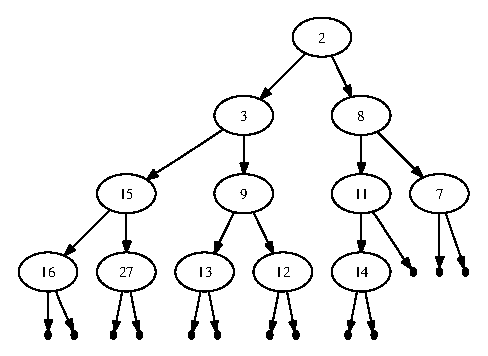
\epsfig{file=../nearly-complete-tree.eps,scale=1.5}

nicht nahezu vollst\"andiger bin\"arer Baum

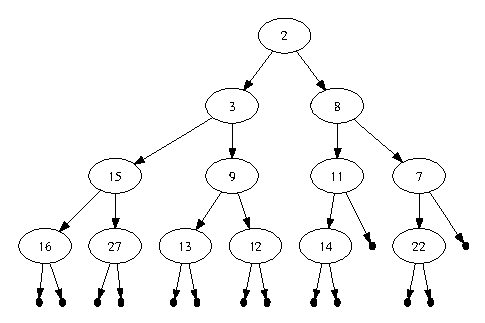
\epsfig{file=../not-nearly-complete-tree.eps,scale=1.5}


\vspace*{\fill}
\tiny \addtocounter{mypage}{1}
\rule{17cm}{1mm}
nahezu vollst\"andige bin\"are B\"aume \hspace*{\fill} Seite \arabic{mypage}
\end{slide}

%%%%%%%%%%%%%%%%%%%%%%%%%%%%%%%%%%%%%%%%%%%%%%%%%%%%%%%%%%%%%%%%%%%%%

\begin{slide}{}
\normalsize

\begin{center}
Die Klasse \texttt{PriorityQueue<E>}
\end{center}
\vspace*{0.5cm}

\footnotesize
wichtig: $\texttt{E} = \textsl{Key} \times \textsl{Value}$
\begin{enumerate}
\item \texttt{boolean offer(E $e$)}

      entspricht  $q.\textsl{insert}(k,v)$. 
\item \texttt{E peek()}

      entspricht $q.\textsl{top}()$
\item \texttt{E poll()}

      entspricht 
      \begin{itemize}
      \item $q.\textsl{top}()$
      \item $q.\textsl{remove}()$
      \end{itemize}
\item \texttt{boolean remove(E $e$)}

      $q.\mathtt{remove}(e)$ entfernt $e$ aus $q$
\end{enumerate}


\vspace*{\fill}
\tiny \addtocounter{mypage}{1}
\rule{17cm}{1mm}
 \hspace*{\fill} Seite \arabic{mypage}
\end{slide}

%%%%%%%%%%%%%%%%%%%%%%%%%%%%%%%%%%%%%%%%%%%%%%%%%%%%%%%%%%%%%%%%%%%%%

\begin{slide}{}
\normalsize

\begin{center}
Huffman-Algorithmus (1952)
\end{center}
\vspace*{0.5cm}

\footnotesize

Anzahl der Buschstaben, $\textsl{count}()$:
\begin{enumerate}
\item $\textsl{leaf}(c,f).\textsl{count}() = f$
\item $\textsl{node}(l,r).\textsl{count}() = l.\textsl{count}() + r.\textsl{count}()$
\end{enumerate}


Anzahl der Bits zur Kodierung eines Strings, $\textsl{cost}()$:
\begin{enumerate}
\item $\textsl{leaf}(c,f).\textsl{cost}() = 0$
\item $\textsl{node}(l,r).\textsl{cost}() = $
      \\[0.2cm]
      \hspace*{1.3cm}
      $l.\textsl{cost}() + r.\textsl{cost}() + l.\textsl{count}() + r.\textsl{count}()$
\end{enumerate}

Start: \quad
$M = \bigl\{ \textsl{leaf}(c_1,f_1), \cdots, \textsl{leaf}(c_k,f_k) \bigr\}$

Zusammenfassen der einzelnen Knoten:
\begin{Verbatim}[ frame         = lines, 
                  framesep      = 0.3cm, 
                  labelposition = bottomline,
                  numbers       = left,
                  numbersep     = -0.2cm,
                  xleftmargin   = 1.3cm,
                  xrightmargin  = 1.3cm,
                  codes         = {\catcode`_=8\catcode`$=3},
                  commandchars  = \\\{\},
                ]
    procedure codingTree(M) \{
        while (#M > 1) \{
            a := minCount(M);
            M := M - \{ a \};
            b := minCount(M);
            M := M - \{ b \};
            M := M + \{ node(a, b) \};
        \}
        return arb M;
    \}
\end{Verbatim} 
%$

\vspace*{\fill}
\tiny \addtocounter{mypage}{1}
\rule{17cm}{1mm}
 \hspace*{\fill} Seite \arabic{mypage}
\end{slide}

%%%%%%%%%%%%%%%%%%%%%%%%%%%%%%%%%%%%%%%%%%%%%%%%%%%%%%%%%%%%%%%%%%%%%%%%%

\begin{slide}{}
\normalsize

\begin{center}
 Berechnung k\"urzester Wege
\end{center}
\vspace*{0.5cm}

\footnotesize
{\em Gewichteter Graph}:  \quad 
 Tripel $G = \langle \nodes, \edges, \weight{\cdot} \rangle$ mit
\begin{enumerate}
\item $\nodes$ ist Menge von \textsl{Knoten}.
\item $\edges \subseteq \nodes \times \nodes$ ist Menge von \textsl{Kanten}.
\item $\weight{\cdot}: \edges \rightarrow \N \backslash\{0\}$ 

      Funktion, die jeder Kante positive \textsl{L\"ange} zuordnet.
\end{enumerate}

\textsl{Pfad} $P$ ist  Liste  $P = [ x_1, x_2, x_3, \cdots, x_n ]$  mit\\[0.3cm]
\hspace*{1.3cm} 
$\forall i \in \{1, \cdots, n-1\}\colon \pair(x_i,x_{i+1}) \in \edges$. 

$\mathbb{P}$:  Menge aller Pfade in $G$

Pfad-L\"ange:  \quad
$\Weight{[x_1,x_2, \cdots, x_n]} \df \sum\limits_{i=1}^{n-1}
\Weight{\pair(x_i,x_{i+1})}$. 

Menge der Pfade, die  $v$ mit  $w$ verbinden: 

 $\paths(v,w) \df \biggl\{ [x_1, x_2, \cdots, x_n] \in \paths \mid  x_1 = v \,\wedge\, x_n = w \}$.

Shortest-Path Funktion \\[0.3cm]
\hspace*{1.3cm} 
 $\spath: \nodes \rightarrow \N$ \\[0.3cm] 
\hspace*{1.3cm} 
 $\spath(v) \df \mathtt{min}\biggl\{ \weight{p} \mid p \in \paths(\source,v) \biggr\}$.


\vspace*{\fill}
\tiny \addtocounter{mypage}{1}
\rule{17cm}{1mm}
K\"urzeste Wege \hspace*{\fill} Seite \arabic{mypage}
\end{slide}

%%%%%%%%%%%%%%%%%%%%%%%%%%%%%%%%%%%%%%%%%%%%%%%%%%%%%%%%%%%%%%%%%%%%%%%%

\begin{slide}{}
\normalsize

\begin{center}
 Eine naive ASM
\end{center}
\vspace*{0.5cm}

\footnotesize
\begin{Verbatim}[ frame         = lines, 
                  framesep      = 0.3cm, 
                  labelposition = bottomline,
                  numbers       = left,
                  numbersep     = -0.2cm,
                  commandchars  = \\\{\},
                  xleftmargin   = 0.0cm,
                  xrightmargin  = 0.0cm
                ]
    \underline{Rule} \textsl{Init}
        \underline{if}  \(\textsl{dist}(\textsl{source}) = \Omega\)
        \underline{then}
            \(\textsl{dist}(\textsl{source})\) := \(0\);
        \underline{endif}
        
    \underline{Rule} \textsl{Run}
        \underline{if} \underline{choose} \(\langle{}u,v\rangle\in\edges\) \underline{satisf}y\underline{in}g
            \(\textsl{dist}(u) \not= \Omega\) \underline{and}  
            \((\textsl{dist}(v)=\Omega\) \underline{or} \(\textsl{dist}(u)+\weight{\langle{}u,v\rangle}<\textsl{dist}(v))\)                 
        \underline{then}
            \(\textsl{dist}(v)\) := \(\textsl{dist}(u)+\weight{\langle{}u,v\rangle}\);
        \underline{endif}
\end{Verbatim}


\vspace*{\fill}
\tiny \addtocounter{mypage}{1}
\rule{17cm}{1mm}
Naive ASM \hspace*{\fill} Seite \arabic{mypage}
\end{slide}


%%%%%%%%%%%%%%%%%%%%%%%%%%%%%%%%%%%%%%%%%%%%%%%%%%%%%%%%%%%%%%%%%%%%%%%%

\begin{slide}{}
\normalsize

\begin{center}
 Moore's Algorithmus
\end{center}
\vspace*{0.5cm}

\footnotesize
\begin{Verbatim}[ frame         = lines, 
                  framesep      = 0.3cm, 
                  labelposition = bottomline,
                  numbers       = left,
                  numbersep     = -0.2cm,
                  commandchars  = \\\{\},
                  xleftmargin   = 0.0cm,
                  xrightmargin  = 0.0cm
                ]
   \underline{Rule} \textsl{Init}
       \underline{if}   \(\textsl{dist}(\textsl{source}) = \Omega\)
       \underline{then} \(\textsl{dist}(\textsl{source})\) := \(0\);
            \(\textsl{mode} := \textsl{scan}\);
            \textsl{fringe} := \(\{ \textsl{source} \}\);
       \underline{endif}
       
   \underline{Rule} \textsl{Scan}
       \underline{if}   \(\textsl{mode}=\mathtt{scan}\) \underline{and} \underline{choose} \(u\in\textsl{fringe}\) 
       \underline{then}
          \({\cal E}\)      := \(\textsl{edges}(u)\);
           \(\textsl{fringe}\) := \(\texttt{fringe} \backslash \{u\}\);
           \(\textsl{mode}\)   := \texttt{relabel};
       \underline{endif}

   \underline{Rule} \textsl{Relabel}
      \underline{if}    \(\textsl{mode} = \textsl{relabel}\)
        \underline{and} \underline{choose} \(\langle{}u,v\rangle\in{\cal{}E}\) \underline{satisfying}  
            \(\textsl{dist}(v)=\Omega\) \underline{or} \(\textsl{dist}(u)+\weight{\langle{}u,v\rangle}<\textsl{dist}(v)\);
      \underline{then}
           \(\textsl{dist}(v)\) := \(\textsl{dist}(u)+\weight{\langle{}u,v\rangle}\);
           \(\textsl{fringe}\;\) := \(\texttt{fringe}\cup\{v\}\);
      \underline{else} 
           \(\textsl{mode}\;\)   := \texttt{scan};
      \underline{endif}
\end{Verbatim}


\vspace*{\fill}
\tiny \addtocounter{mypage}{1}
\rule{17cm}{1mm}
Moore's Algorithmus \hspace*{\fill} Seite \arabic{mypage}
\end{slide}


%%%%%%%%%%%%%%%%%%%%%%%%%%%%%%%%%%%%%%%%%%%%%%%%%%%%%%%%%%%%%%%%%%%%%%%%

\begin{slide}{}
\normalsize
\vspace*{-2.5cm}

\begin{center}
 Dijkstra's Algorithmus
\end{center}
\vspace*{-0.8cm}

\footnotesize
\begin{Verbatim}[ frame         = lines, 
                  framesep      = 0.3cm, 
                  labelposition = bottomline,
                  numbers       = none,
                  numbersep     = -0.2cm,
                  commandchars  = \\\{\},
                ]
\underline{Rule} \textsl{Init}
    \underline{if}   \(\textsl{dist}(\textsl{source}) = \Omega\)
    \underline{then} 
         \(\textsl{Fringe}.\textsl{insert}(0,\textsl{source})\);
         \textsl{dist}(\textsl{source}) := \(0\);
         \textsl{Visited}      := \(\{ \textsl{source} \}\);
         \textsl{mode}         := \textsl{scan};
    \underline{endif}
    
\underline{Rule} \textsl{Scan}
    \underline{if}     \(\textsl{mode} = \textsl{scan}\)
       \underline{and} \underline{not} \texttt{Fringe}.\texttt{isEmpty}()  
    \underline{then}
        \(\langle{d,u}\rangle\) := \textsl{Fringe}.\textsl{top}();
        \textsl{Fringe}.remove();
        \textsl{Visited} := \(\textsl{Visited} \cup \{ u \}\);
       \({\cal E}\,\)    := \(\textsl{edges}(u)\);            
        \(\textsl{mode}\;\) := \texttt{relabel};
    \underline{endif}

\underline{Rule} \textsl{Relabel}
    \underline{if} \(\textsl{mode} = \textsl{relabel}\)           \underline{and}  
       \underline{choose} \(\langle{}u,v\rangle\in{\cal{}E}\) \underline{satisfying}  
           \(\textsl{dist}(v)=\Omega\) \underline{or} \(\textsl{dist}(u)+\weight{\langle{}u,v\rangle}<\textsl{dist}(v)\);
    \underline{then}
        \(\textsl{dist}(v)\) := \(\textsl{dist}(u)+\weight{\langle{}u,v\rangle}\);
        \underline{if} \(\textsl{dist}(v) = \Omega\) \underline{then}
            \(\textsl{Fringe}\) := \(\texttt{Fringe}.\textsl{insert}(\langle\textsl{dist}(v),v\rangle)\);
        \underline{else}
            \(\textsl{Fringe}\) := \(\texttt{Fringe}.\textsl{change}(\langle\textsl{dist}(v),v\rangle)\);
        \underline{endif} 
    \underline{else} 
        \(\textsl{mode}\;\) := \texttt{scan};
    \underline{endif}
\end{Verbatim}

\vspace*{\fill}
\tiny \addtocounter{mypage}{1}
\rule{17cm}{1mm}
Dijkstra's Algorithmus \hspace*{\fill} Seite \arabic{mypage}
\end{slide}

%%%%%%%%%%%%%%%%%%%%%%%%%%%%%%%%%%%%%%%%%%%%%%%%%%%%%%%%%%%%%%%%%%%%%%%%

\begin{slide}{}
\normalsize

\begin{center}
Die Monte-Carlo-Methode
\end{center}

\footnotesize
\begin{enumerate}
\item Idee:  Problem durch zuf\"allige Simulation l\"osen
\item Anwendungen
      \begin{enumerate}
      \item Berechnung komplexer Volumina oder allgemein mehrfacher Integrale
      \item Verhalten eines Systems h\"angt von zuf\"alligen Einfl\"ussen ab

            Beispiel: U-Bahn, Anzahl der Passagiere schwankt zuf\"allig
      \item Berechnung von Wahrscheinlichkeiten beim \\
            Gl\"uckspiel

            Gewinn-Wahrscheinlichkeit bei Poker
      \item Historisch: Konstruktion der ersten Atom-Bombe
      \end{enumerate}
\end{enumerate}

Beispiele in der Vorlesung
\begin{enumerate}
\item Berechnung von $\pi$
\item Berechnung zuf\"alliger Permutationen 

      Anwendung: Gewinn-Wahrscheinlichkeiten beim \\
      Texas Hold'em
\end{enumerate}

Merkmale:
\begin{enumerate}
\item gut geeignet f\"ur grobe Absch\"atzungen
\item aufwendig f\"ur hohe Genauigkeit
\end{enumerate}


\vspace*{\fill}
\tiny \addtocounter{mypage}{1}
\rule{17cm}{1mm}
Monte-Carlo-Methode \hspace*{\fill} Seite \arabic{mypage}
\end{slide}



\end{document}

%%% Local Variables: 
%%% mode: latex
%%% TeX-master: t
%%% End: 
